\label{sec:3_methodology}

\begin{comment}
This chapter may have many names. Lately, many have named it "Methodology", but names like "Design and Implementation", a "name" of a developed system, etc. are also often used. Just find a name that matches your research. Regardless, the important thing here is to describe YOUR research.

INTRO: Again, start the chapter with a sentence or two explaining why you have this chapter (repeating the last sentences from the proposed summary in the previous chapter) - assuming that some readers have not read the previous chapter.

MIDDLE SECTIONS: What are your ideas? Your solutions. How have you done "things"? Implementation details. Frameworks used. Etc. Also, discuss alternative ways of doing things and explain why you have chosen to do things as you have. WHAT! HOW! WHY!

SUMMARY: End this chapter with a summary section. Summarize what you have done and why! Main knowledge gained. What have we learned? Lead to the next chapter, stating that you will test your prototype.
\end{comment}


% INTRO:
% Again, start the chapter with a sentence or two explaining why you have this chapter (repeating the last sentences from the proposed summary in the previous chapter) - assuming that some readers have not read the previous chapter.


%This chapter will introduce some methods that address some of the challenges presented in this chapter. 
In this chapter, the two methods proposed in this work are presented in more detail. The overall goal of these two methods is to explore how different machine learning models can implement explanatory methods in various domains that still provide value to the user. Different model architectures represent data in different ways. 
This chapter highlights how insights into these representations can give a researcher or user a new understanding of the data and models used.
Both models presented in this chapter have multimodal capabilities, specifically in visual and linguistics. The way they achieve this multimodality differs. 

The first model uses a classical \gls{vqa} architecture, with the addition of the \gls{flex} framework. 
Using this framework, the model can label feature maps in the \gls{cnn} to get information from the visual domain translated into natural language. The explanation originates, therefore, from the visual domain, translated into text. 


The second method introduces a large language model (LLM) combined with a standard \gls{cnn}. The image features of the \gls{cnn} get translated into text, and the explanation happens in the text domain. 

Therefore, these two models discussed in this chapter will investigate explanations originating from different domains.

%The other model also describes images using text but is based on a large language model. The next chapter is, therefore, a summary of methods used to answer the research goals of this thesis.

% MIDDLE SECTIONS:
    % Implementation
    \section{FLEX-VQA}

    This section will delve deeper into implementing the first proposed method, FLEX-VQA. The name originates from the framework FLEX, originally introduced by Wickramanayake et al. \cite{wickramanayakeFLEXFaithfulLinguistic2019}, combined with visual question and answering (VQA). 
    
    \label{sec3:flex_vqa}
        \subsection{Overview}
        % What:

        % FLEX
        To make \gls{vqa} models easier to understand for the user, the explanation can originate from either of the two modalities of the model, either the language model, the image model, or both. 
        The method presented in this experiment will address this task using the cross-modality explanation method \gls{flex}. An overview of the \gls{flex} model has already been described shortly in sub-chapter \ref{sec:2_related_work} on page \pageref{sec:2_related_work}. This method is relevant to this method because it explains the network's visual reasoning of why a picture should be in a given class using natural language. The \gls{flex} framework combines a \gls{cnn}, which is pretrained on the specific task and does not need any further training that alters the \gls{cnn} to give it explainable abilities. An overview of the original \gls{flex} framework can be seen in Figure \ref{fig:flex_overview}.

        \begin{figure}[htb]
            \centering
            \centerline{
            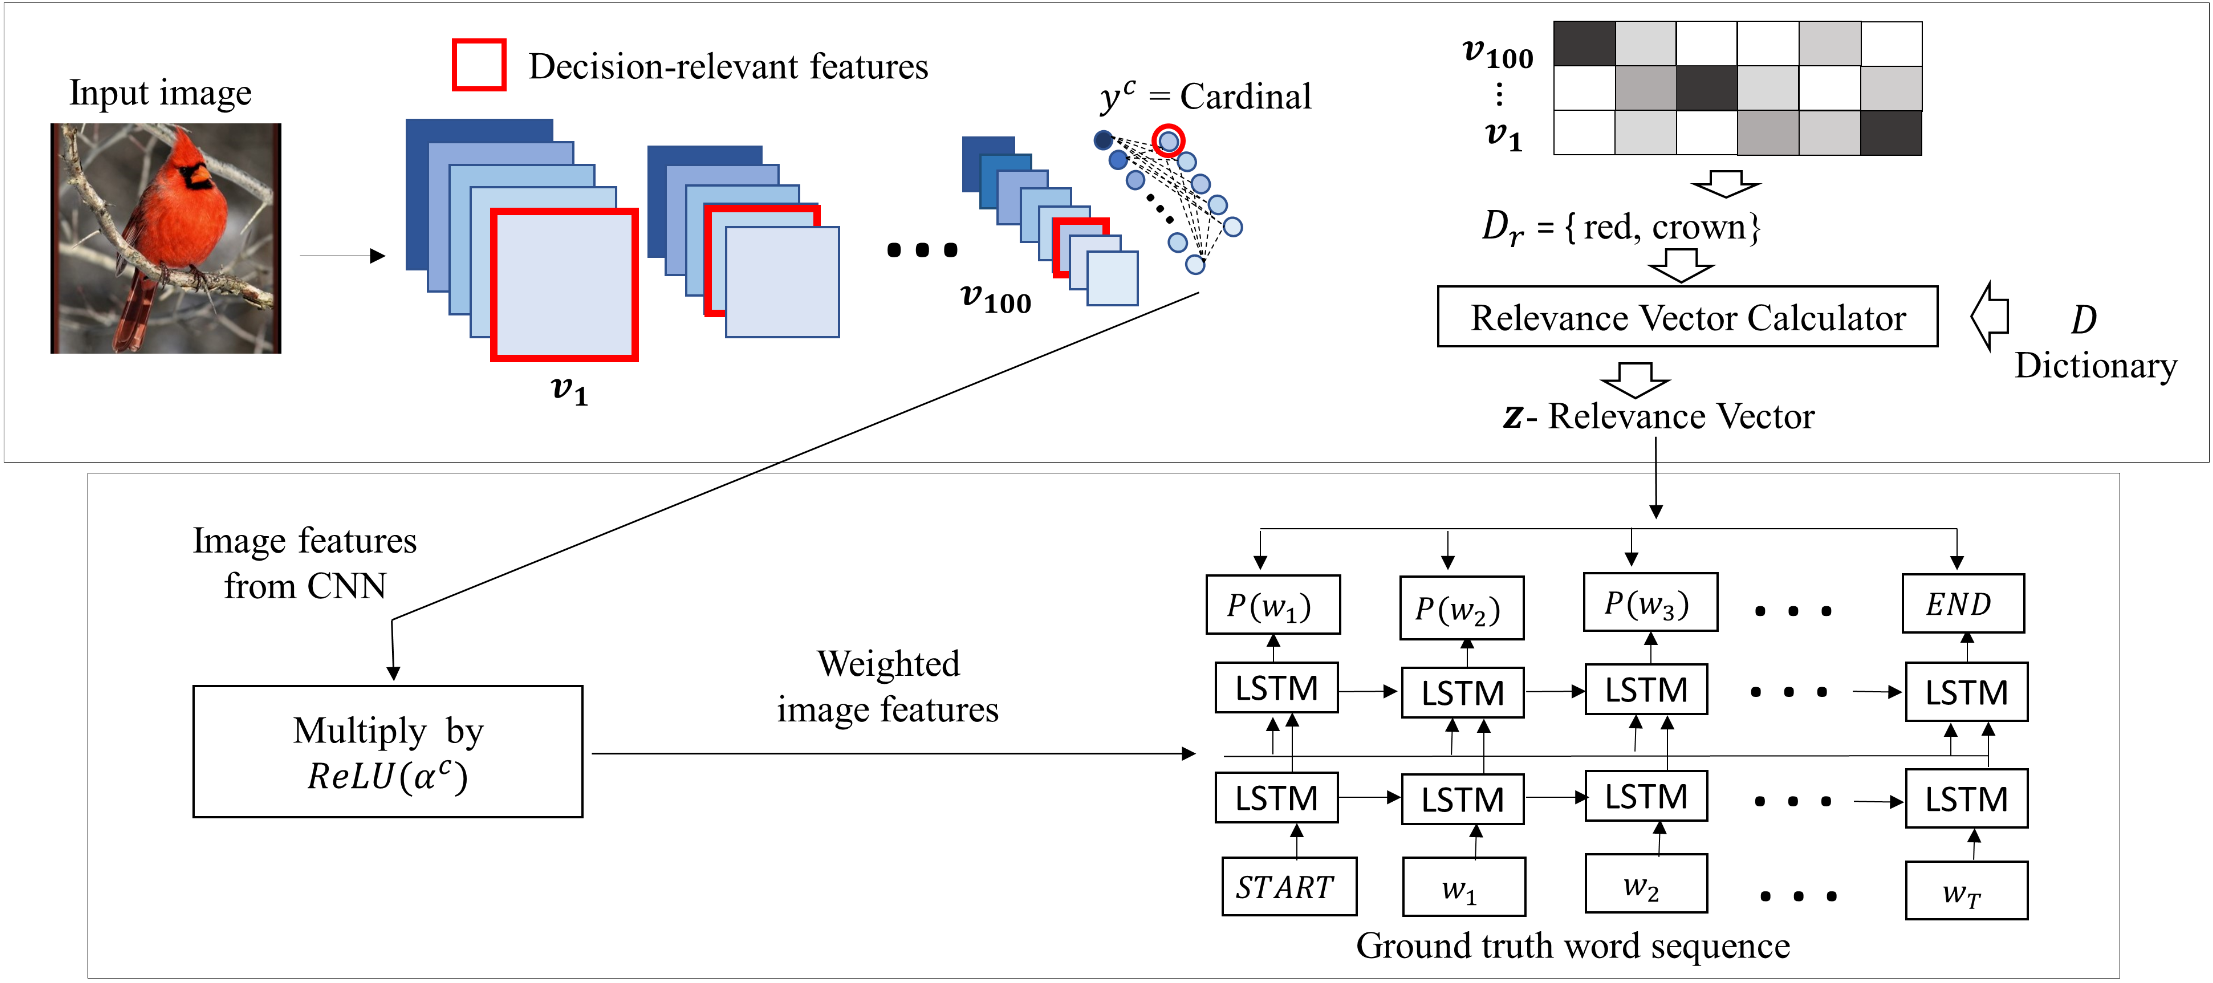
\includegraphics[width=17cm]{images/FLEX_overview.png}}
            \caption[Overview of the FLEX Framework.]{Overview of the FLEX Framework.\\
            Figure credit: Wickramanayake et al. \cite{wickramanayakeFLEXFaithfulLinguistic2019}.}
            \label{fig:flex_overview}
        \end{figure}

        \subsection{The motivation for this method}

        % Why:
        By using \gls{flex} as a starting point, the purpose of the method in this experiment is to adapt it to have \gls{vqa} abilities. In order to make this adaption, the dataflow shown in Figure \ref{fig:flex_architecture_proposal} is proposed. Using this technique, a user can get an answer for a question regarding an input image that is both in natural language and faithful to the underlying \gls{cnn} model, making it more explainable and transparent. The explanation is faithful to the underlying model since it uses the actual gradients in the \gls{cnn} to find the words used to answer the question. 
        This feature ensures that if the underlying \gls{cnn} model has learned features that correlate with the answer but are not the intended or logical features to pay attention to, these flaws get communicated to the user. Making a model that can explain what it considers important to a user, also when flawed, is important when making a system where a user can make a factually based decision in trusting the answer.
        

        % More in detail on how FLEX works. 
        \subsection{Original FLEX in more detail}
        \label{sec3:flex_detailed}
        First, the \gls{flex} framework works by having a \gls{cnn} predict the class of an input image. Given the image and its predicted class $c$, the method finds a subset of the most important feature maps from each layer in the pretrained \gls{cnn}. To find the global activation score of each feature map, it sums up each neuron in the layer and then repeats this process for each layer in the \gls{cnn}. After that, it sorts the layers in order of importance and chooses a subset of $n$ layers so that the subgroup has a combined importance over a predefined threshold. When a subset of the most important visual features is collected, \gls{flex} connects these visual features with linguistic features. 

        \gls{flex} uses the \gls{gradcam} technique proposed by Selvaraju et al. \cite{selvarajuGradCAMVisualExplanations2020} to do a backward pass through the feature maps of the \gls{cnn} to find the largest class activation maps when predicting a class. This information is then used to map words to important visual feature extractions in the network. This mapping of words combines the separable feature layers salient layers of the \gls{gradcam} method with natural language to make better explanations.
        
        The way \gls{flex} archives explainability is to find a connection score between a word ($w$) to the elements of the important feature maps ($F$) so that the word ($w$) best describes the important visual element ($v$) in each feature map. With a given natural language description of the ground truth ($D_I$) of an image ($I$), \gls{flex} uses the corresponding description for every image and builds a dictionary that contains all words in every description seen in the training data. This dictionary ($D$) is used when describing new images during testing. 
        Creating this combined dictionary is conceptually similar to how language models generate a dictionary of tokens used for tokenization.
        For each word ($w$) \gls{flex} calculates the co-occurrence score for each feature ($v \in F$), using the Dice score \cite{diceMeasuresAmountEcologic1945, sorensenMethodEstablishingGroups1948}, as seen in Equation \ref{eq:dice_score_flex}. The word with the highest co-occurrence score gets associated with the visual feature ($v$). 
        
        \begin{equation}
            \textit{score}(w, v) = \frac{2 \times \textit{occur}(w, v)}{\textit{count}(w) + \textit{count}(v)}
        \label{eq:dice_score_flex}
        \end{equation}

        When the dictionary $D_I$ for each image and the dictionary for all images $D$ is computed, the dictionary for the individual class labels can be found. This class label dictionary ($D_c$) contains the combined dictionary of each image of a specific class and can be defined as $D_c = \bigcup D_I$, where the class label of $I$ is $c$. 
        Lastly, the dictionary $D_r$ is the words extracted recursively from the \gls{cnn}. When an image is provided, and the class is predicted, \gls{flex} starts at the last convolutional layer and finds the top-$k$ features from that layer and their associated words. This collection of associated words from feature maps is done recursively until the first convolutional layer is reached, and the union of all these words is named $D_r$.


        To describe decision-relevant features, \gls{flex} computes the relevance of a word $w$ to each of the dictionaries using the formula in Equation \ref{eq:relevance_calculation_flex}, where $D_x$ is a placeholder for $D_r$, $D_I$, and $D_c$.

        \begin{equation}
            \operatorname{relevance}\left(w, D_x\right)=\left\{\begin{array}{cl}
            0 & w \notin D_x \\
            -\log \left(\frac{\left|D_x\right|}{|D|}\right) & \text { otherwise }
            \end{array}\right.
            \label{eq:relevance_calculation_flex}
        \end{equation}

        When the relevance scores for each dictionary are calculated, the relevance vector $z$ is defined as in Equation \ref{eq:relevance_vector_flex}:

        \begin{equation}
            z = (g(w1), g(w2), ..., g(w\left|D\right|))
        \label{eq:relevance_vector_flex}
        \end{equation}

        Where $w_i$ is the $i^{th}$ word in $D$ and
        \begin{equation*}
            g(w_i) = relevance(w_i, D_r) + relevance(w_i, D_I ) + relevance(w_i, D_c)
        \end{equation*}
  

        To train the framework to generate a textual description, \gls{flex} uses two stacked LSTMs, where the first LSTM receives the ground truth word $w_{t-1}$. The second LSTM gets the hidden state of the first LSTM, concatenated with the visual feature vector from the \gls{cnn}. The output of the second LSTM is encoded to vocabulary space to produce a conditional probability distribution, defined as:

        \begin{equation}
            P (w_{t-1} | w_{\le t-1}, I)
        \label{eq:flex_contitional_proba_func}
        \end{equation}
        
        This distribution samples the current word $w_t$ at time step $t$.  
        The relevance vector $z$ is element-wise multiplied by this probability distribution to produce the relevance loss and is defined as:

        \begin{equation}
            \operatorname{loss}\left(w_t, I\right)=\max \left(\boldsymbol{z} \odot P\left(w_t \mid w_{\leq t-1}, I\right)\right)
        \end{equation}

        When no ground truth label is available during interference, \gls{flex} samples from the conditional distribution in Equation \ref{eq:flex_contitional_proba_func} to get the next word then passed as the input to the LSTM in the next step.
                

   
        This labeling of visual features can be reminiscent of DenseCap proposed by Johnson et al. \cite{johnsonDenseCapFullyConvolutional2016}, and Neural Baby Talk proposed by Lu et al. \cite{luNeuralBabyTalk2018}. The main difference between these methods and \gls{flex} is that \gls{flex} can be added to a network after the architecture is finalized, trained, and evaluated. In theory, the framework is agnostic to the underlying network. However, one limitation is that the visual encoder must have a property in which distinct parts of the image activate distinct parts of the network. 
        
        
        

        \subsection{Implementation}
        % How:
        Given that \gls{flex} can combine information from the visual domain with natural language, it is an exciting framework to explore in the field of \gls{xai} and \gls{vqa}. A modified architecture to \gls{flex} is presented in this thesis, as seen in Figure \ref{fig:flex_architecture_proposal}. This proposed architecture has unfortunately not been tested because of technical hindrances outside the scope of this work. A more detailed explanation of these hurdles is described in subsection \ref{subsec:no_flex}. However, since much of the available time for this thesis was spent researching this approach and solving the hurdles, an overview of the architecture will still be provided in this section.


        % Dataset: VQA 1.0 vs. 2.0
        \subsubsection{Dataset: VQA 1.0 and COCO}
        The dataset chosen for this experiment is the VQA 1.0 dataset \cite{agrawalVQAVisualQuestion2016} instead of the more balanced VQA 2.0 \cite{goyalMakingVQAMatter2017}. 
        This experiment's goal is not to achieve state-of-art accuracy but to test the validity of this method. The VQA 1.0 dataset allows the \gls{vqa} model to learn biases in the data that will be utilized in this method. Because of its unbalance, the authors of the VQA 1.0 dataset propose to use a k-way classification with 1000 classes. The rationale behind this decision is that the top thousand classes cover 82.67\% of all the train and validation answers. Optimizing this way makes the assignment no longer open-ended but a more straightforward task by choosing one class out of a thousand. 
        
        This optimization will make the answer easier to compute, reducing training time and making it easier to control if the prediction is correct. Another benefit of this simplification is that the FLEX-VQA method can use the answer as a class, making it more efficient to adapt it to the \gls{flex} framework. This is because the \gls{flex} method builds a dictionary for each class ($D_c$). 
        In order to make the dictionary $D_c$, the method will need descriptions for each image. 
        Another benefit of using the VQA dataset is that the images originate from the Common Object in Context (COCO) dataset \cite{linMicrosoftCOCOCommon2015}. This dataset is a large-scale object detection, segmentation, and captioning dataset, meaning that the images in the VQA dataset are already described in COCO. 
       

        % Input from essay here.
        \subsubsection{Proposed architecture}
        \label{sec3:proposed_architecture}
        
        Figure \ref{fig:flex_architecture_proposal} shows how the data flow in the proposed method is supposed to work. It closely follows the original \gls{flex} architecture, with adaptations to make it answer questions. It consists of a \gls{cnn} that extracts visual information and a 2-layered \gls{lstm} \cite{hochreiterLongShorttermMemory1997} \gls{rnn} that combine linguistic information with extracted visual features. 
        The \gls{cnn} used in this implementation is the same as in the original framework, which is a modified VGG-16. The modification is a technique proposed by \cite{gaoCompactBilinearPooling2016} et al. called Compact Bilinear Pooling, which reduces feature dimensionality without sacrificing performance. This ensures a more efficient and faster training and inference time, which also has the potential benefit of reducing the risk of overfitting.


        
        
        % Explain the proposed data flow/architecture 
        % VQA
        
        The wanted requirements of the system will need to be defined before any method can be developed. 
        The method should be able to have an image as input alongside a question related to the content of this image. The wanted output is a locally accurate answer to the question and a description that is also locally accurate to the model. 
        
        \textbf{\\The VQA model\\} 
        The proposed architecture can be utilized to make a model and pipeline that achieves the required features. The proposed method consists of a standard \gls{vqa} model with a k-way classification optimization. This architecture is essentially the same as the one presented in the original VQA 1.0 paper, called \textit{deeper LSTM Q + norm I}, which achieves an accuracy of 57.75\% on the complete test set. 
        This network comprises an image pipeline (\textit{norm I}) with activations from the \gls{cnn} being $l_2$ normalized. The question pipeline (\textit{deeper LSTM Q}) consists of an \gls{lstm} with two stacked layers. 
        The image embeddings are then transformed to a dimensionality to match the question embeddings. This is done by a fully-connected layer, which makes the image features a vector with a length of 1024.

        When the image and question features have the exact dimensions, they are merged by pointwise multiplication. 
        This fusion vector is then passed through a fully connected neural network with two hidden layers, 1000 hidden units in each layer, and a dropout of 0.5.
        Finally, the answer with the best fit is found by passing the result of the  fusion vector through a SoftMax layer to predict the final class.
        
        
        
        
        

        % FLEX
        \textbf{\\FLEX\\}
        Since the \gls{vqa} system is now a classification task, it can be matched with the \gls{flex} framework. 
        The importance score is recursively calculated using the image features in each feature map of the \gls{cnn}. The formula used in this calculation is shown in Equation \ref{eq:flex_activaiton_score}, where $Z$ is the total number of neurons in the feature map $A$, the predicted label for class $c$ is $y^c$ and $a_{ij}$ is the $ij^{th}$ neuron in $A$.

        \begin{equation}
            \alpha^c = \frac{1}{Z} \sum_i \sum_j \frac{\partial y^c}{\partial a_{ij}} 
        \label{eq:flex_activaiton_score}
        \end{equation}


        In order to remove negative influence and only evaluate scores contributing to the specific class, the importance scores $\alpha^c$ are then multiplied with a \gls{relu}. These positive-only activation scores are then fed into the secondary stacked LSTM of the \gls{flex} framework, which also gets the hidden state from the first LSTM. This stacked LSTM network is separate from the LSTMs of the \gls{vqa} system, as it is trained only to output descriptions, whereas the one in the \gls{vqa} is used to encode the question features. 
        The rest of the \gls{flex} framework is the same as described in Section \ref{sec3:flex_detailed}. The main difference between the original \gls{flex} and this method is that instead of the \gls{cnn} predicting a class, the classification method now predicts an answer using the \gls{vqa} model.
        
        
        
        % Training
        \textbf{\\Training and testing\\}
        Given that \gls{flex} is a post-hoc explanation method, it does not need to be trained simultaneously as the \gls{vqa} system. This separation ensures that the \gls{vqa} system can be trained separately from the explanation system and, thereby, can be tuned to achieve satisfactory accuracy before the explanation system is introduced.
        However, even though the systems are separate, the explanations are still connected directly from the extracted image features and, therefore, will be locally accurate to the \gls{cnn} method.

        % Train VQA
        In order to train the \gls{vqa} system, the input image with corresponding questions and their ground truth answers is supplied. The VQA 1.0 dataset contains all these image-question-answer pairs and will be used in this experiment.
        Then entire \gls{vqa} model is trained end-to-end using a cross-entropy loss, as described in the VQA 1.0 paper, where it was presented originally.

        % Train FLEX
        The \gls{flex} is a separate model that is outside of the \gls{vqa} model and, therefore, will need to be trained after the implemented \gls{vqa} method is fully trained. Some optimizations can still be implemented to make this training process faster. The optimization, with a considerable impact on training time, is to precompute the image features when the \gls{vqa} system is trained. Because \gls{flex} uses the image features for each image together with the predicted answer, these can be saved during \gls{vqa} training so that they do not need to be fed through the \gls{vqa} model once more.


        To train the \gls{flex} framework to the task at hand, it must have extracted image importance scores, a ground truth description of the image from the COCO dataset, and the predicted answer for the question. 
        The answer is, in this experiment, regarded as the class label and, therefore, needed when \gls{flex} makes the dictionary $D_c$. The dictionary $D_I$ contains the image description, and the relevance dictionary $D_r$ is calculated using the importance scores from the \gls{cnn}.

        While testing the combined system, the \gls{vqa} method still needs an image and related questions. Then the predicted answer is made by the fully connected network. This answer defines the class dictionary $D_c$ that the \gls{flex} framework uses when making a conditional probability distribution. This distribution contains the combined relevance defined by $z$, which is a function of the relevance for $D_c$, $D_I$, and $D_r$, as described in Equation \ref{eq:relevance_vector_flex} in Section \ref{sec3:flex_detailed}.

        The \glspl{lstm} gets trained by feeding each word in the ground truth caption into the first layer alongside the hidden state of the \gls{lstm}. This is used to compute the next state, which gets concatenated with relevant activation scores from the \gls{cnn} and is input to the second and last, \gls{lstm}-layer. 
        The output from the second \gls{lstm}-layer is encoded to vocabulary space to make a conditional probability distribution that will later be used to calculate the probability of predicting that word, given the provided image features. The word with the highest probability is chosen and used as input in the first layer of the LSTM.
        This word prediction is repeated until the stop word is predicted. 
        


    
            
        \begin{comment}
            During the training of the method proposed in this thesis, an image and its corresponding questions and answers from the \gls{vqa} dataset are used as input. The images are fed through a \gls{cnn}-network, which can be pretrained on a larger dataset, such as ImageNet \cite{dengImageNetLargeScaleHierarchical2009}. This is because the explaining method utilizes feature maps in each layer of the \gls{cnn}, so it is agnostic on what type of \gls{cnn} it is and what dataset it is trained on earlier. The \gls{cnn} predicts a class of what it sees in the image and, with a backward pass, finds important feature maps in each  convolutional layer. Each feature in the set of important feature maps gets associated with a word and stored in a relevance vector. This process is done by computing a co-occurrence score between each word in the ground truth caption and the feature. The feature with the highest co-occurrence score gets linked with that feature. 
        
                % LSTM
             
            
                % Testing
            The architecture takes an image and an optional question as input during prediction. The \gls{cnn} extracts important features in the layers, which get fed into the \gls{lstm}. 
            
            If no question is input to the algorithm during prediction, the model will use the most accurate predicted answer caption that describes the image as a whole as a caption for the image. On the other hand, if a question is submitted alongside the image, the \gls{lstm} will generate captions that answer the question asked and then chose the most decision-relevant answer as the caption. 
        \end{comment}
        
        
        
        
        % Data flow
        \begin{figure}[htb]
            \centering
            
            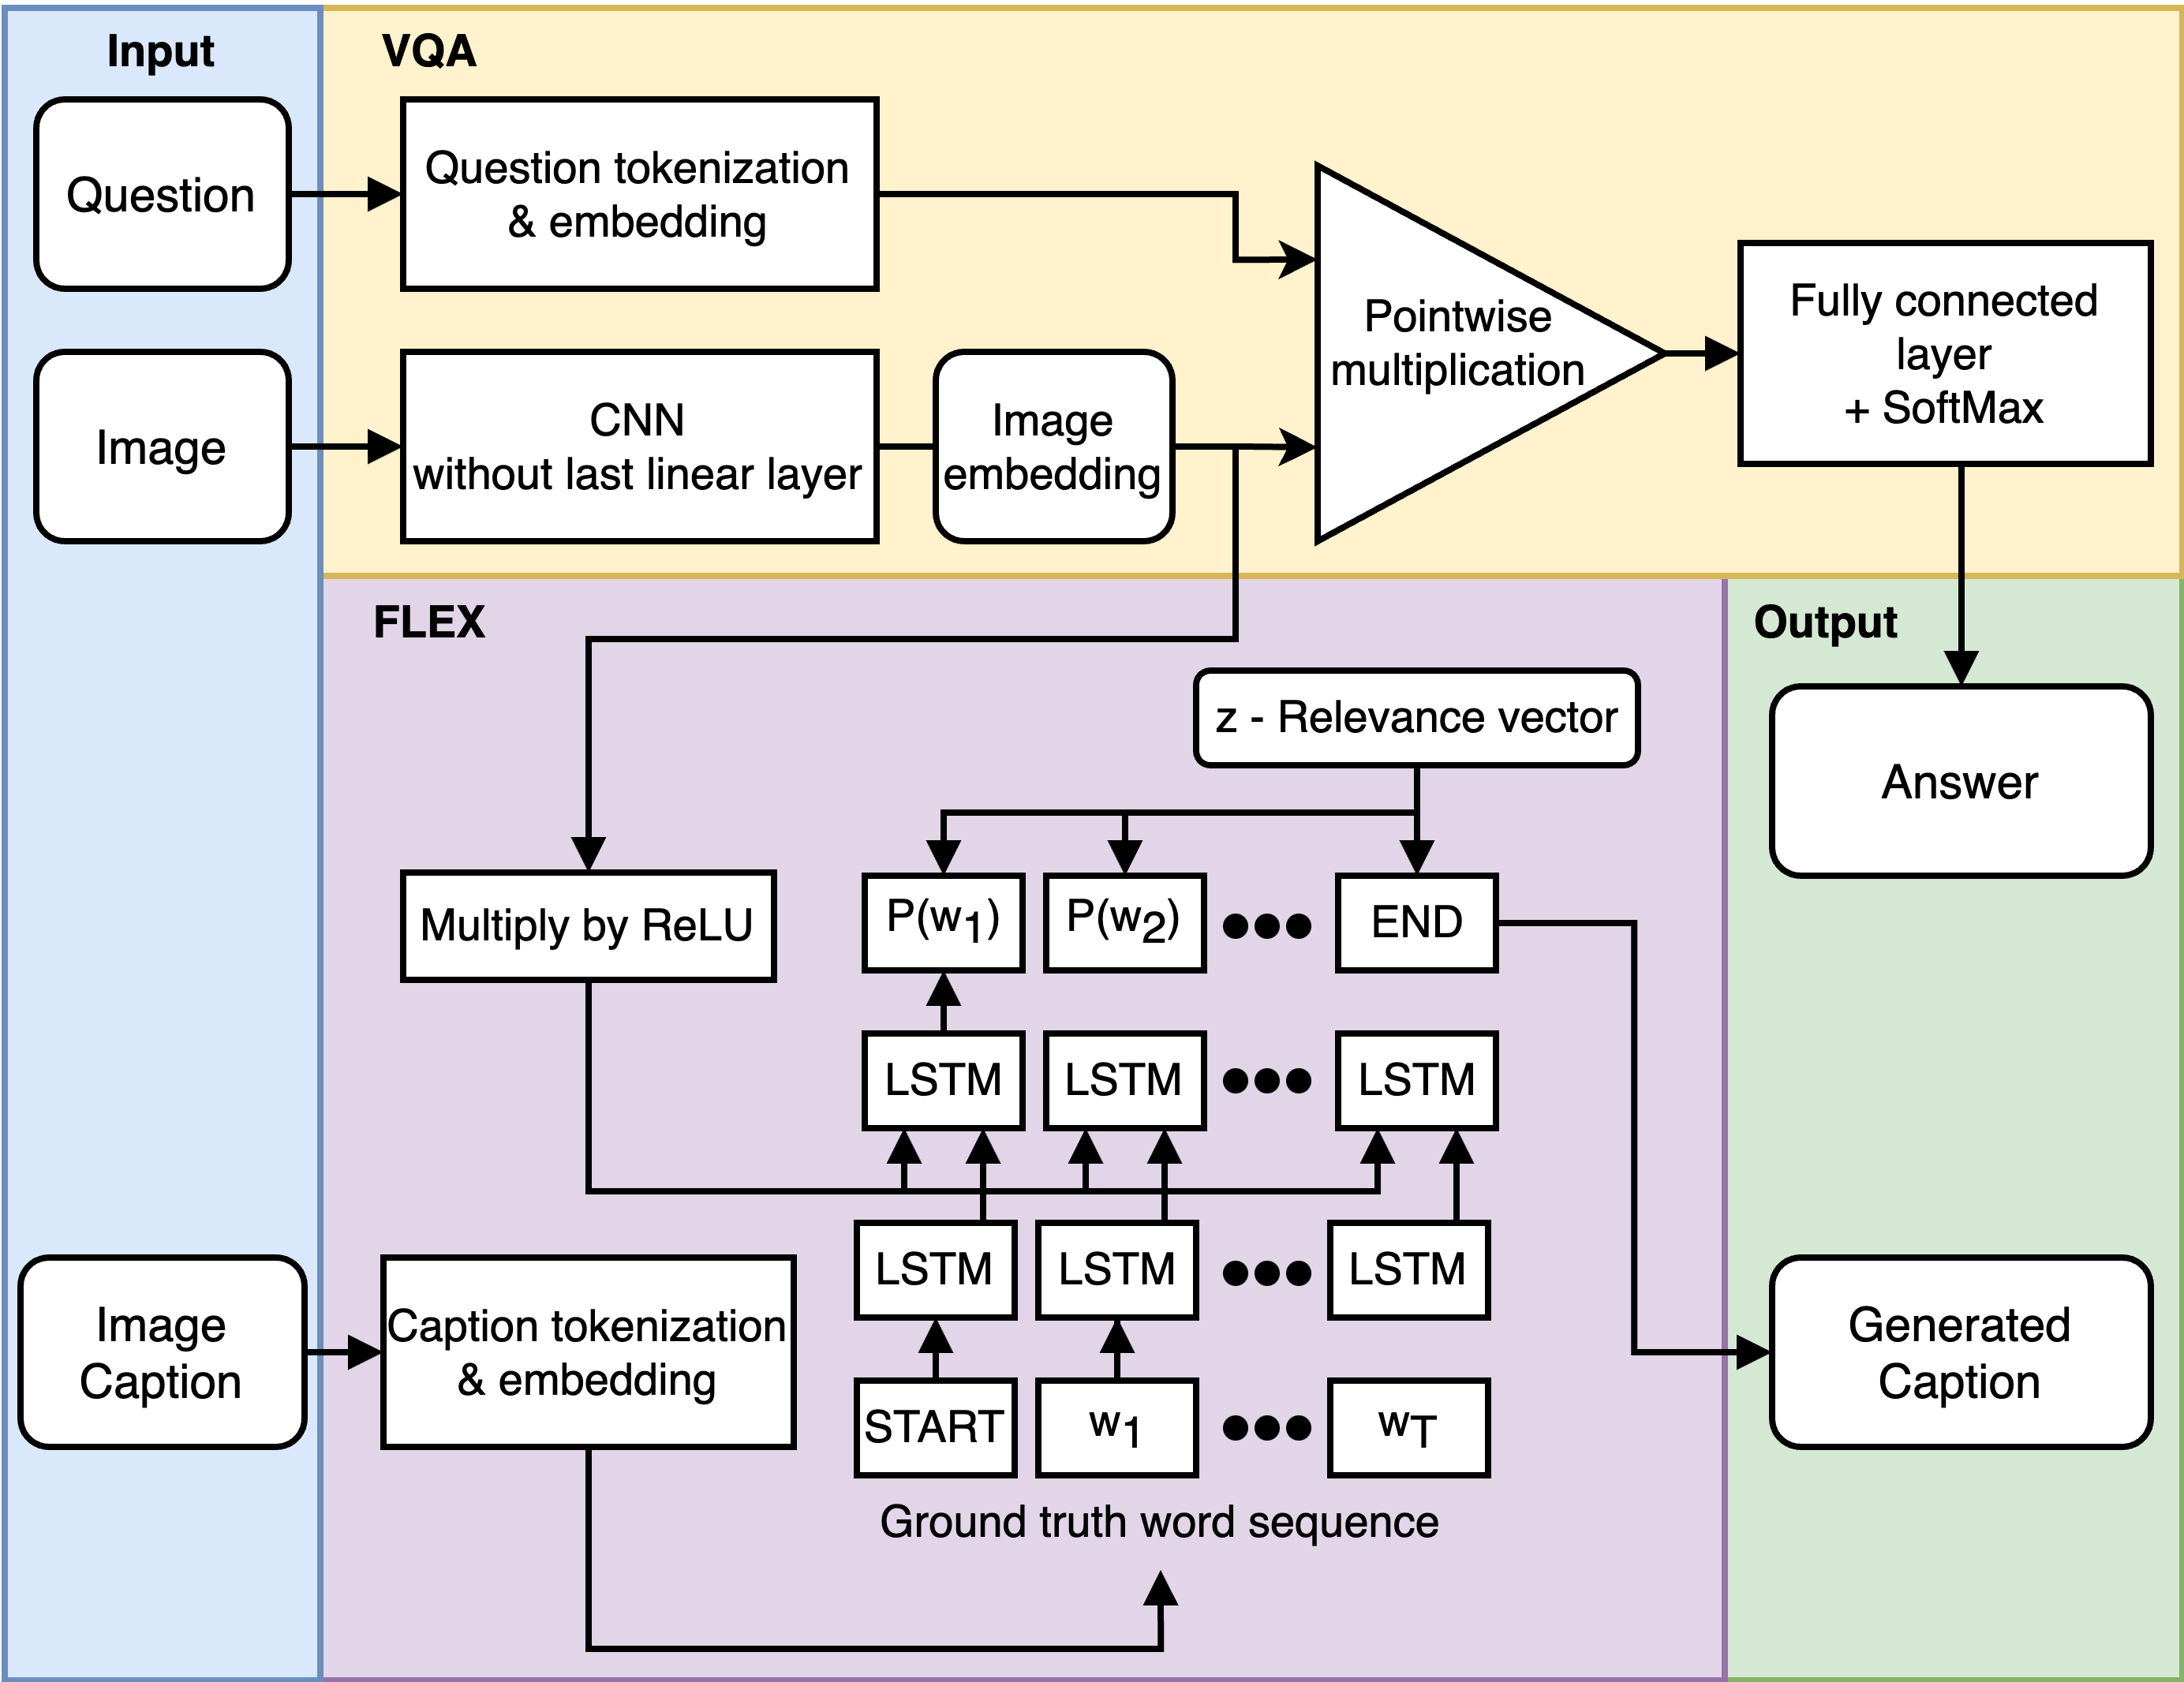
\includegraphics[width=\linewidth]{images/flex_architecture_proposal.png}
            \caption{Proposal of the data flow and components explored in this experiment.
            %Figure by the author.
            }
            \label{fig:flex_architecture_proposal}
        \end{figure}
                
                
        

        
        
        \begin{comment}
            Neither the \gls{cnn} nor the \glspl{lstm} needs to be specifically trained to be explainable. 
            The architecture uses the underlying nature of the models to build a transparent answer to the underlying model and explains to the user what the model values as important. 
    
            
            However, in order to make the method work for a specific case, the \gls{cnn} has to be trained or fine-tuned to the specific dataset. This is because \gls{flex} uses the predicted class to build a dictionary of words for each class. 
        
            If the specific dataset has few images available for training, it can be pre-trained on a larger dataset, like ImageNet, and fine-tuned to the specific dataset. By using this pre-training, the \gls{cnn} can benefit from transfer learning so that general concepts and features can be learned from a general dataset, and valuable data samples for the specific task can learn the fine-grained features specific to this task.
    
            The original \gls{flex} framework uses the LSTMs to generate descriptions based on associated words from activated neurons. In order to make this framework accept question-answer pairs, the LSTMs are trained on questions and ground-truth pairs instead of descriptions. The theory is that a system trained on this question-answer (QA) pairs will still provide the model with an understanding of the objects in images to make a description. 
            For this theory to work, the QA pairs will need to be structured so that the model can learn about objects, locations of objects, time of actions, who is doing the action, why the action is performed, and how the action is performed. An example of a dataset that fulfills these descriptions is the Visual7W dataset, introduced by Zhu et al. \cite{zhuVisual7WGroundedQuestion2016}. 
        \end{comment}
        
        



        \subsection{Why this method has no results}
        \label{subsec:no_flex}

            % Intro
            To implement the proposed architecture as shown in Figure \ref{fig:flex_architecture_proposal}, it was natural to use the original code from the \gls{flex} paper as a starting point.
            The authors of the \gls{flex} paper also released the code used to do the experiments in the article on GitHub\footnote{https://github.com/sandareka/FLEX} to encourage others to iterate on their method. The original experiments use a \gls{cnn} called Compact-Bilinear Pooling, a classifier proposed by Gao et al. \cite{gaoCompactBilinearPooling2016}. While the FLEX framework is designed to be model agnostic, the actual implementation of the experiments is tied closely with the \gls{cnn}, which proved to be a hurdle when trying to recreate the results in the paper and expand on the architecture and features. 
            This method mainly does not provide finished experiments or results because an outdated machine learning framework makes compact-bilinear pooling \gls{cnn} practically impossible to execute. 
            Combined with the tight integration between the implemented \gls{flex} method and the \gls{cnn} method, considerable resources have been put into separating these two methods, customizing the software, and building containers around it, with no success.
    
            
            \paragraph{The original implementation of FLEX\\}
            For \gls{flex} to work, it needs to get important features from the \gls{cnn}. This is an essential part of the framework and therefore needs insight into how the layers of the \gls{cnn} are structured.
            The implemented version of the original \gls{flex} architecture uses the Compact-Bilinear Pooling \gls{cnn}, which in short, uses kernelization to reduce the number of dimensions of bilinear features to make it more computationally efficient at the cost of having an architecture that deviates somewhat from a more traditional \gls{cnn} architecture. Therefore, the authors of the \gls{flex} paper have implemented a version of the framework that addresses these special considerations when calculating co-occurrence metrics between words and features. 
        

            \paragraph{Why Caffe was needed\\}
            % Why Caffe was needed
            To use the same \gls{cnn} as the original \gls{flex} in a new context, as in this experiment, would require retraining or fine-tuning this network to suit the images in the given dataset. This would require the Compact-Bilinear Pooling model to train using the new pictures in the specific dataset. Alternatively, a new \gls{cnn} could be chosen that could be merged with the \gls{flex} framework. The original Compact-Bilinear Pooling came with pretrained weights from training on the Caltech-UCSD Birds (CUB) \cite{PeronaLabCUB2002011} dataset. This dataset has images from Flickr and ImageNet containing a subset solely focused on bird species and a relatively small amount of photos (11,788, compared to 14 million images in ImageNet \cite{dengImageNetLargeScaleHierarchical2009}). Therefore, the original weights are best fit to classify this CUB dataset and will require retraining outside this specific task.
            Because of how the original \gls{flex} framework is structured, it would need to be substantially rewritten for a new \gls{cnn} to be used in place of the Compact-Bilinear Pooling. Therefore the best way forward was to use this \gls{cnn}, like the original method.

            \paragraph{Getting Caffe to run\\}
            % Getting Caffe to run
            To train the Compact-Bilinear Pooling on a new dataset, the underlying machine learning framework it was built in had to be installed.
            This framework is named Caffe and is a deep learning framework developed by Berkeley AI Research (BAIR) / The Berkeley Vision and Learning Center (BVLC). It's a precursor to the framework  Caffe2, which was initially built by Facebook and is now merged with PyTorch. Because Caffe was forked into Caffe2, the development of the original stagnated. Developers implemented new features and compatibility in Caffe2, while the original Caffe has not received an update since 2017. 
            Because of the rapidly evolving nature of software and hardware since 2017, it proved to be a nontrivial task to get Compact-Bilinear Pooling written in Caffe to run on the hardware available during this project.
            The \gls{flex} framework is implemented in TensorFlow version 1.7, which is also considered outdated at the time of writing. However, in contrast to Caffe, the teams at TensorFlow have made tools and helpers to run outdated code and translate it into current versions.


            To get the compute benefits necessary for deep learning, the Caffe framework will need to run on \glspl{gpu}.
            The framework supports \glspl{gpu} from Nvidia with \gls{cuda} version 5 through 8 \cite{CaffeInstallation, CaffeDeepLearning}, as well as AMD \glspl{gpu}. The \glspl{gpu} in the compute cluster available to run experiments for this thesis are Nvidia RTX 2080 Ti, Nvidia A100, and AMD Vega 10 XL/XT, which run \gls{cuda} version 11.7, 11.5 and ROCm version 4.5.0 respectively \cite{MLNodesUniversitetet}. 
            The mismatch between Caffe's highest supported \gls{cuda} version and the version available on the hardware need to be addressed.
            To not break compatibility with other services on the compute cluster, containerization was needed. Luckily containers are being actively deployed with  Caffe versions with \gls{gpu} support, most notably from Nvidia and AMD.


            At the time the implementation of the architecture started, communication was established with the IT staff at the University of Oslo, which is responsible for the available computing cluster.
            
            At that stage, only an experimental implementation of containerization was available through the container engine Podman \cite{Podman}. Using this container engine, the Nvidia container could not attach the Nvidia \glspl{gpu}. However, the AMD ROCm container could access the AMD \glspl{gpu}. Unfortunately, this AMD container did not have the correct driver compatibility to train the \gls{cnn}. Since Podman did not result in a container that could run successfully, a different container engine was installed, namely Apptainer, formerly known as Singularity. This new engine could see all the Nvidia \glspl{gpu}, but not the AMD ones. After the initial errors were ironed out, a Caffe container from Nvidia was successfully installed. Although successfully installed, the container had trouble running the training examples in the \gls{flex} code repository. 
            When an error message was solved, a new one arose.
            Therefore no definite problem could be addressed, but rather several error messages pointing to possible driver incompatibility. 
            The most likely explanation for the error messages was an incompatibility issue between the Caffe version in the container and the hardware it was tested on. After extensive testing and error-solving in seven months, the decision was taken that this technical problem was outside the scope of this experiment, and this method was discontinued for this project. 
            
            \begin{comment}
                KOMMET HIT!!
            \end{comment}
            
            \paragraph{How these problems could have been mitigated\\}
            % How this could be fixed.
            % implemented from scratch. 

            The main limitation of the chosen approach was getting the Caffe framework to work. However, the proposed method could still be implemented with a new approach. 
            Because this method could bring new insight into how \gls{vqa} systems are interpreted, exciting experiments could still be carried out.
            Some suggested improvements based on the experience gained implementing this method are:

            \begin{itemize}
                \item \textbf{Remove Caffe from FLEX\\} 
                To have better compatibility with modern hardware and be more accessible for research moving forward, discontinued frameworks should be updated with more up-to-date versions. At the time of publishing the \gls{flex} paper (2019), the development of the Caffe framework had already been stale for two years. To facilitate peer review and additional implementations so that the proposed methodology can be further developed, researchers benefit from publishing material for others to follow and implement themselves. 
                Removing the Caffe framework from the \gls{flex} framework makes the method more accessible and easier for others to expand on.

                \item \textbf{Update FLEX to TensorFlow 2\\}
                The FLEX framework is implemented in TensorFlow version 1.7, released in 2018. As of writing this thesis, TensorFlow versions 1.x are considered legacy. However, version 1.15, the latest version 1.x, is supported by TensorFlow 2 through a legacy helper. By updating to a more recent version, the framework can implement more modern features and optimizations, gain compatibility with modern hardware and acquire more users already familiar with the current versions. This upgrade can speed up the implemented \gls{flex} framework through software and hardware optimizations and speed up the development of the framework itself. 
                TensorFlow has migration guides and scripts to help translate from version 1 to 2 \cite{MigrateTensorFlowTensorFlow}, which makes the migration manageable. 
    

                \item \textbf{Make FLEX model agnostic in practice\\}
                Theoretically, the \gls{flex} framework is separate from the \gls{cnn}. As proposed in the paper where the framework is introduced, the implementation of the \gls{flex} framework would benefit from being adapted to be agnostic to the underlying method. The initially implemented method has methods to extract image features specific to the \gls{cnn} used, making it dependent on that particular model. Using an agnostic implementation of the gradient search through the \gls{cnn} feature maps, the method could be extended by allowing testing different \glspl{cnn} to extract features and find co-occurrences with linguistic features. This could make implementing the technique for new \glspl{cnn} easier and make more methods explainable. 

            \end{itemize}

        % Outro / summary
        \subsection{Summary of FLEX-VQA}
        To summarize, by implementing the \gls{flex} framework into a \gls{vqa} method, the combined framework would make interpreting \gls{vqa} models easier and locally accurate. \gls{flex} has the same benefits as \gls{lime} of being locally accurate and model agnostic. Having insight into a locally accurate explanation model would make it possible for researchers and users of an implemented system to see if the underlying model is trustworthy based on what the model deems important. 

        Unfortunately, no experiments were conducted with this method due to technical difficulties. However, the process described in this section still provides insight into how an interpretable and locally accurate \gls{vqa} system could be designed. 
        The main takeaways from this section are how a framework could be designed to extract visual explanations in the visual domain described in the linguistic field. The \gls{flex} framework searches through the \gls{cnn} and finds important features that are then described using natural language. 

        The following section will introduce an experiment where, in contrast to the previous, the visual features are first translated to the linguistic domain and explained using linguistic explanation techniques.

    \section{Alpaca-VQA}
    \label{sec3:alpaca_vqa}

    The experiment in this section will explore an approach to design an \gls{llm} that can interpret images, reason about their content, and be able to answer general text questions. 
    There are many ways a multimodal \gls{llm} could be developed, but this experiment aims to have a system with an explanation method in the linguistic domain. The rationale is that the previous experiment, described in Section \ref{sec3:flex_vqa}, was explained in the visual domain and translated into text. The investigation in this section will do the opposite. The image features are extracted and translated to text, where the explanation system works on the text directly. 

    This section presents the implementation details of a VQA version of the Alpaca model. First, an overview of the reasons for choosing Alpaca for this experiment will be given. A more detailed description and rationale for the specific implementation of this model are then discussed, such as how the model has gained visual capabilities and how image features are implemented into the language model.


        \subsection{Overview}
        % What:
        To make an \gls{llm} that can see the world and explain what it sees, it was outside the scope of this experiment to train an \gls{llm} from scratch, both regarding time and resources. When training, an \gls{llm} requires vast quantities of good-quality data. Training the model requires large compute clusters that consume lots of energy, cost much to facilitate, and produce unwanted greenhouse emissions. Therefore, an \gls{llm} that was already pretrained was needed for this experiment to be fine-tuned further to answer the research goals. 
        


        % Alpaca-LoRA
        \subsubsection{Alpaca-LoRA}
        Even though the Stanford Alpaca model was trained using significantly less computing power compared to other \glspl{llm}, it is still advantageous to further lower the necessary compute budget to train and fine-tune models. A technique that was proposed by Hu et al. called \gls{lora} \cite{huLoRALowRankAdaptation2021} addresses this issue. This technique manages this task by adding pairs of rank-decomposition weight matrices, commonly called update matrices, on the current weights and only trains these newly added weights. This approach has many advantages, most importantly accelerating the training while reducing memory consumption. Other benefits of these added matrices are that the original weights are kept frozen, making the \gls{lora} model less prone to catastrophic forgetting. This catastrophic forgetting can happen when large connectionist networks, like deep neural networks for \glspl{llm}, are trained on multiple tasks in sequence. In these scenarios, the models are prone to forgetting the earlier tasks \cite{mccloskeyCatastrophicInterferenceConnectionist1989}. Having the original weights available in a frozen state while training on a new task keeps the learned representations, as they are not changed. The added weights are typically less than 10 percent of the original trainable parameters, making training domain-specific models more feasible and faster. 
        Because the fine-tuned matrices are so small, these \gls{lora} weight matrices can be changed on the fly depending on the task. 
        This allows for a system where a large base model pretrained on an extensive text corpus, with smaller \gls{lora} matrices, is fine-tuned to different needs that still benefit from the larger base model when giving answers.
        When using \gls{lora} matrices, they also allow training and interference on consumer hardware, like regular desktop \glspl{gpu}. It is even possible to do interference on a single-board computer like the Raspberry Pi, although at a significant speed decrease \cite{artemandreenko[@miolini]VeSucefullyRunned2023}. 


        \subsection{Implementation}
        % What I did implement
        To address the research questions stated in \ref{sec:1_2_problem_statement}, considering ??, a \gls{lora} version of the Stanford Alpaca version was used to carry out the experiments. The code used as a starting point was a fork of Erik J. Wang's Alpaca-LoRA \cite{wangAlpacaLoRA2023}, which was further modified to fit the experiments in this section. 
        The most notable modification to this model is to make it cross-modal by allowing it to take both text and images as input.


        

        \subsubsection{Make a language model see images}
        % How to get the model to see
        An image encoder had to be implemented to enable the model to interpret images. To allow the \gls{llm} to analyze image data, the visual features had to be extracted and translated into the linguistic domain, which could be merged with the input prompt. 
        To make a system that more efficiently can change image encoders without changing the \gls{llm}, the design of the image-to-text method is to encode features as text strings.
        The proposed dataflow is shown in Figure \ref{fig:alpaca_vision}. This architecture allows the language model to be agnostic to the image encoder, allowing it to use a \gls{cnn} or vision transformer that is fine-tuned to the task.

        % Data flow
        \begin{figure}[htb]
            \centerline{
            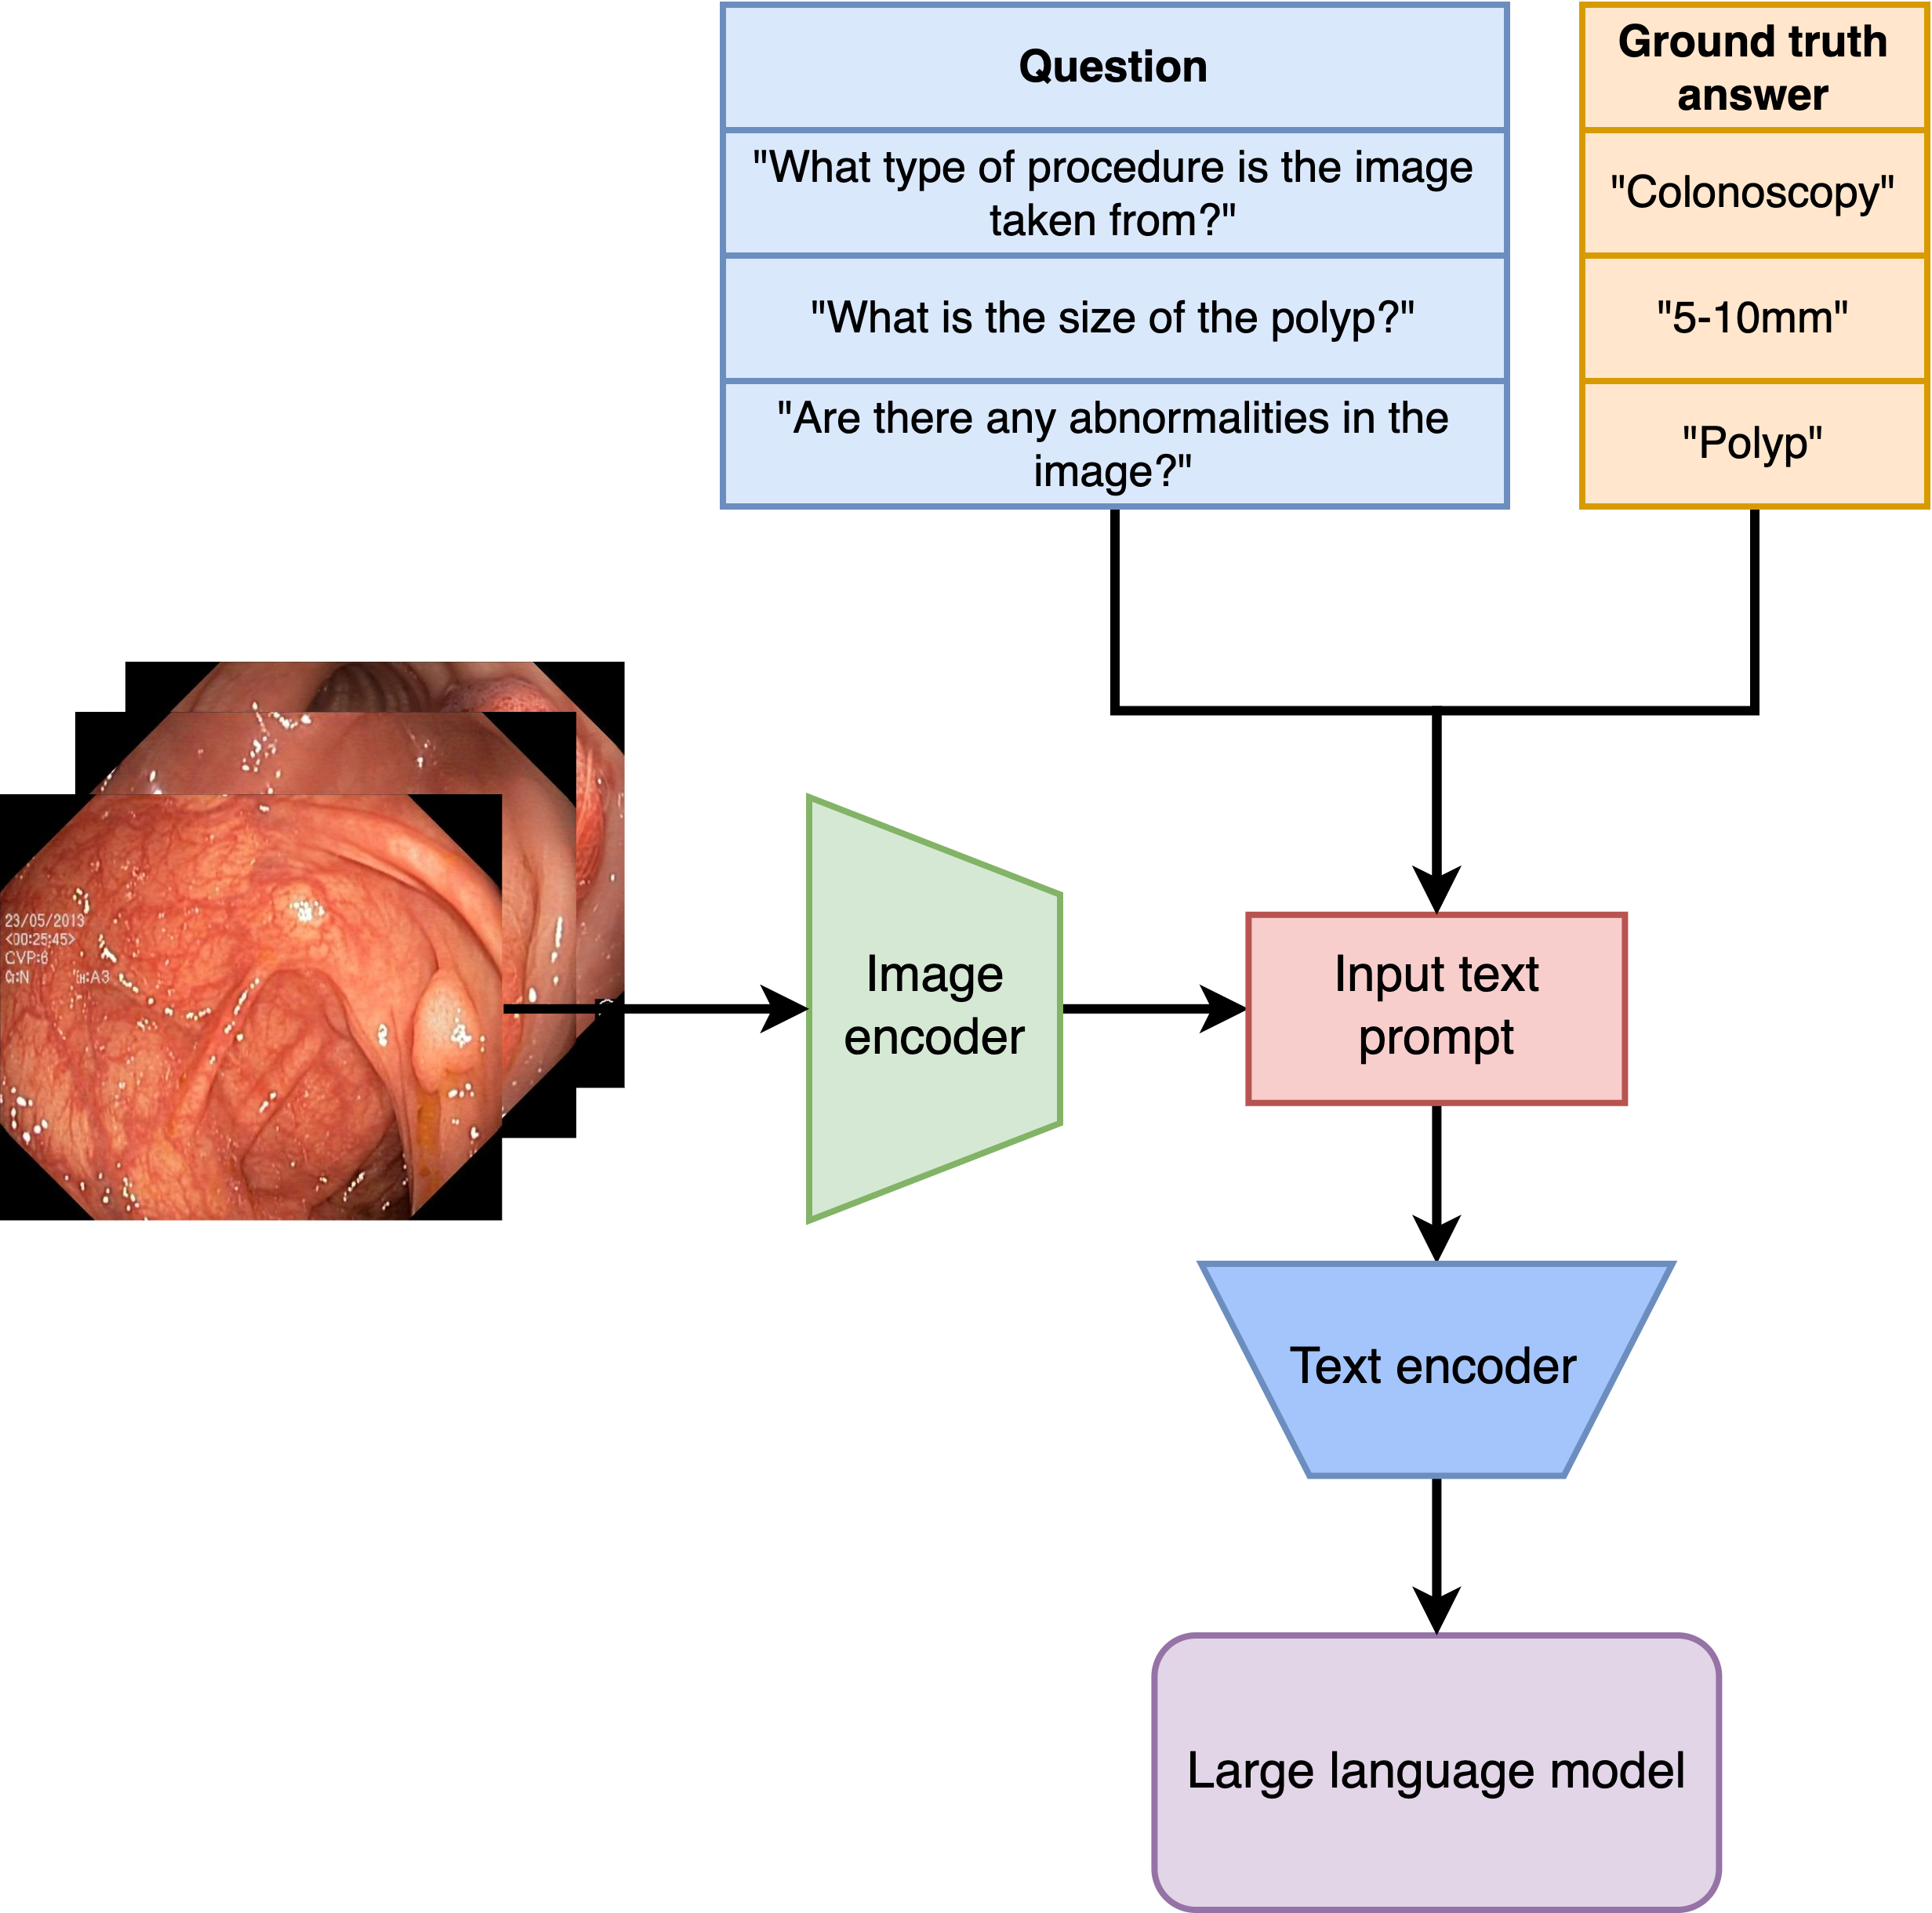
\includegraphics[width=\textwidth]{images/alpaca_vision.png}}
            \caption[Overview of the proposed dataflow to make large language models interpret images.]{Overview of the proposed dataflow to make large language models interpret images. The images in this Figure are from the HyperKvasir dataset by Borgli et al. \cite{borgliHyperKvasirComprehensiveMulticlass2020}. The rest of the diagram is by the author of this work.}
            \label{fig:alpaca_vision}
        \end{figure}


        % How & Why :
        Specifically, the image encoder first implemented was \gls{vgg}-16, proposed by Simonyan and Zisserman at Oxford \cite{simonyanVeryDeepConvolutional2015}. The reason for implementing this \gls{cnn} is that it is a known network that performs relatively well on the ImageNet dataset, where the correct label is in the predicted top five in 90.38\% of the samples in the test set \cite{Vgg16TorchvisionMain}. The VGG-16 model used for the experiments is pre-trained on the ImageNet \cite{dengImageNetLargeScaleHierarchical2009} dataset. The model presumably performs better if pretrained on the specific dataset used, namely the HyperKvasir dataset \cite{borgliHyperKvasirComprehensiveMulticlass2020} introduced by Borgli et al. However, the experiments will explore the proposed approach's feasibility rather than achieve optimal accuracy.

        % Explain why VGG-16 should work even if it does not give regions of interest
        Given that the \gls{vgg}-16 network is pre-trained on ImageNet, it outputs a probability for each of the 1000 classes in the dataset. To address the task of extracting valuable features from any image regardless of whether the \gls{cnn} has been pre-trained for the task, the method implemented extracts features(?) from the 100 ImageNet classes with the highest probability. With this approach, the image feature extraction will find a consistent number of features in an image, sorted with the feature with the highest probability first. The features with the highest probability will likely have a feature map similar to the predicted class in ImageNet. Therefore, even if the class label from ImageNet is not connected with a correct label from the HyperKvasir dataset, there is a high likelihood that the feature extraction will still be practical to extract image features.

        The \gls{vgg}-16 \gls{cnn} was initially developed for the image classification task, not object classification. It consists of multiple convolutional layers followed by fully connected layers, and it does not have any built-in mechanisms for handling \gls{roi} operations. 
        Therefore, since \gls{vgg}-16 is designed as an image classifier, it only outputs the classes it recognizes in the image as a whole, which means it does not perform particularly well for localization tasks. Object classifiers, like R-CNN \cite{girshickRichFeatureHierarchies2014}, Faster R-CNN \cite{renFasterRCNNRealTime2015}, and variants of YOLO \cite{redmonYouOnlyLook2016, redmonYOLO9000BetterFaster2016, redmonYOLOv3IncrementalImprovement2018, bochkovskiyYOLOv4OptimalSpeed2020, jocherYolov5, liYOLOv6SingleStageObject2022, wangYOLOv7TrainableBagoffreebies2022, jocherYOLOUltralytics2023}, among others are made to output \gls{roi}, which would allow the image encoder also to encode locations of detected objects within the image. These object classifying qualities from an image encoder will most likely give the \gls{llm} image data of a higher quality to work from. However, the experiments will test the feasibility of the implementation using \gls{vgg}-16.

        % More info on the other image encoder

        
        \paragraph{Images to text prompt\\}
        % How to encode images into text
        To encode the image features into a format that the \gls{llm} can interpret, the image features must be converted into a form that can be embedded into a natural language question-and-answer format. The dataset used to train the Stanford Alpaca model follows a \textit{question-input-answer} format, as shown in Figure \ref{fig:alpaca_prompt_format}. This format is structured so that the question comes first, followed by an optional input to the prompt with detailed information that can be used to answer the question. Additional up-to-date information can therefore be embedded in the text prompt if the model's training set does not contain information to answer the question. This input function enables the \gls{llm} to answer new questions even after completing the training.
        
        To make the new task of interpreting images while keeping the prompt text format close to the original, image features are incorporated into the \textit{input} section of the original prompt. By not changing the original structure of the prompt, the model is better suited to utilize the knowledge gained from the pre-training. The feasibility of incorporating image features in text prompts has been successfully explored by Yang et al. in the paper MM-REACT \cite{yangMMREACTPromptingChatGPT2023}. 
        The team explores methods to make ChatGPT a multimodal model, including interpreting images.
        The MM-REACT model achieves this by encoding images using an X-Decoder model proposed by Zou et al. \cite{zouGeneralizedDecodingPixel2022}. This model features \gls{roi} capabilities using dense captioning, which outputs class labels and coordinates of the corners of bounding boxes. These extracted features are then concatenated into a text string that the \gls{llm} receives as an input prompt. 
        The modified Alpaca model used in this experiment uses a similar approach to the one in MM-REACT by encoding image features as text. When using the \gls{vgg}-16 model, the final text prompt to the Alpaca-LoRA model is the same as shown in Figure \ref{fig:alpaca_modified_prompt_format}.
        
        % Original prompt format
        \begin{figure}[htb]
            \centerline{
            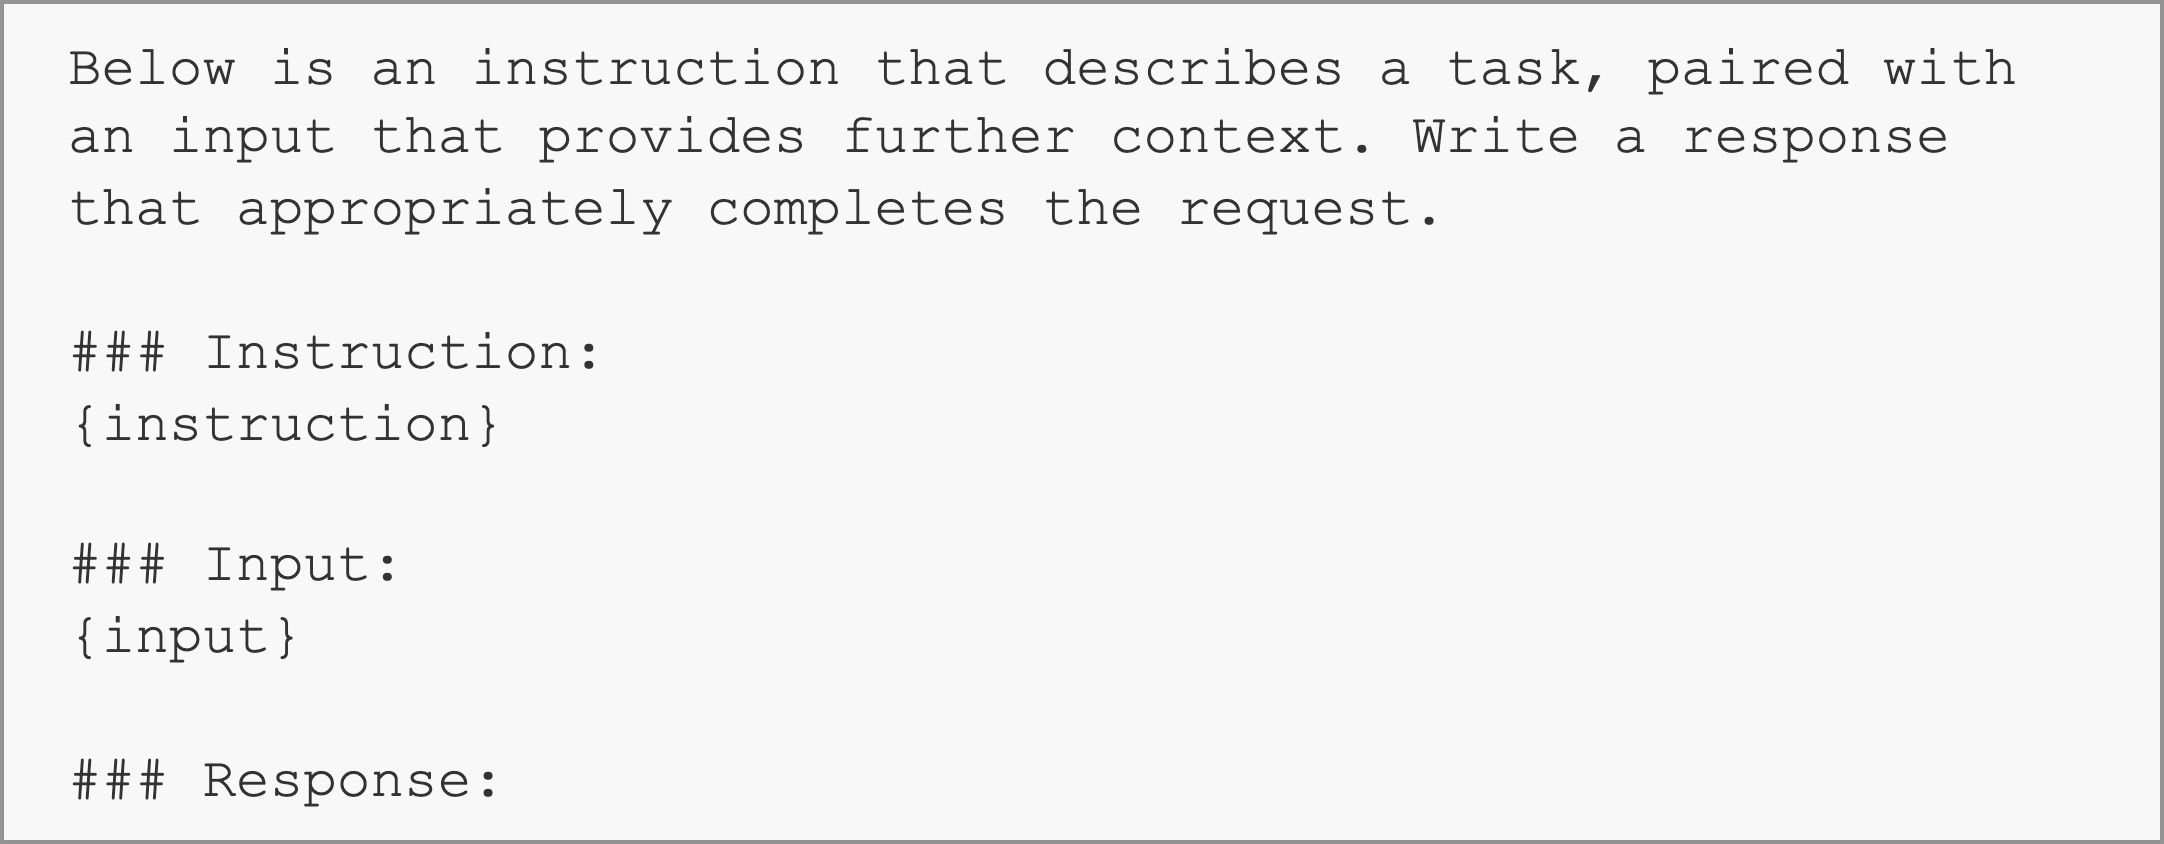
\includegraphics[width=\textwidth]{images/alpaca_prompt_format.png}}
            \caption[Overview of the original text prompt to the Stanford Alpaca model, with additional input.]{Overview of the original text prompt to the Stanford Alpaca model \cite{taoriStanfordCRFM, taoriStanfordAlpacaInstructionfollowing2023}, with additional input.}
            \label{fig:alpaca_prompt_format}
        \end{figure}

        % Modified prompt format
        \begin{figure}[htb]
            \centerline{
            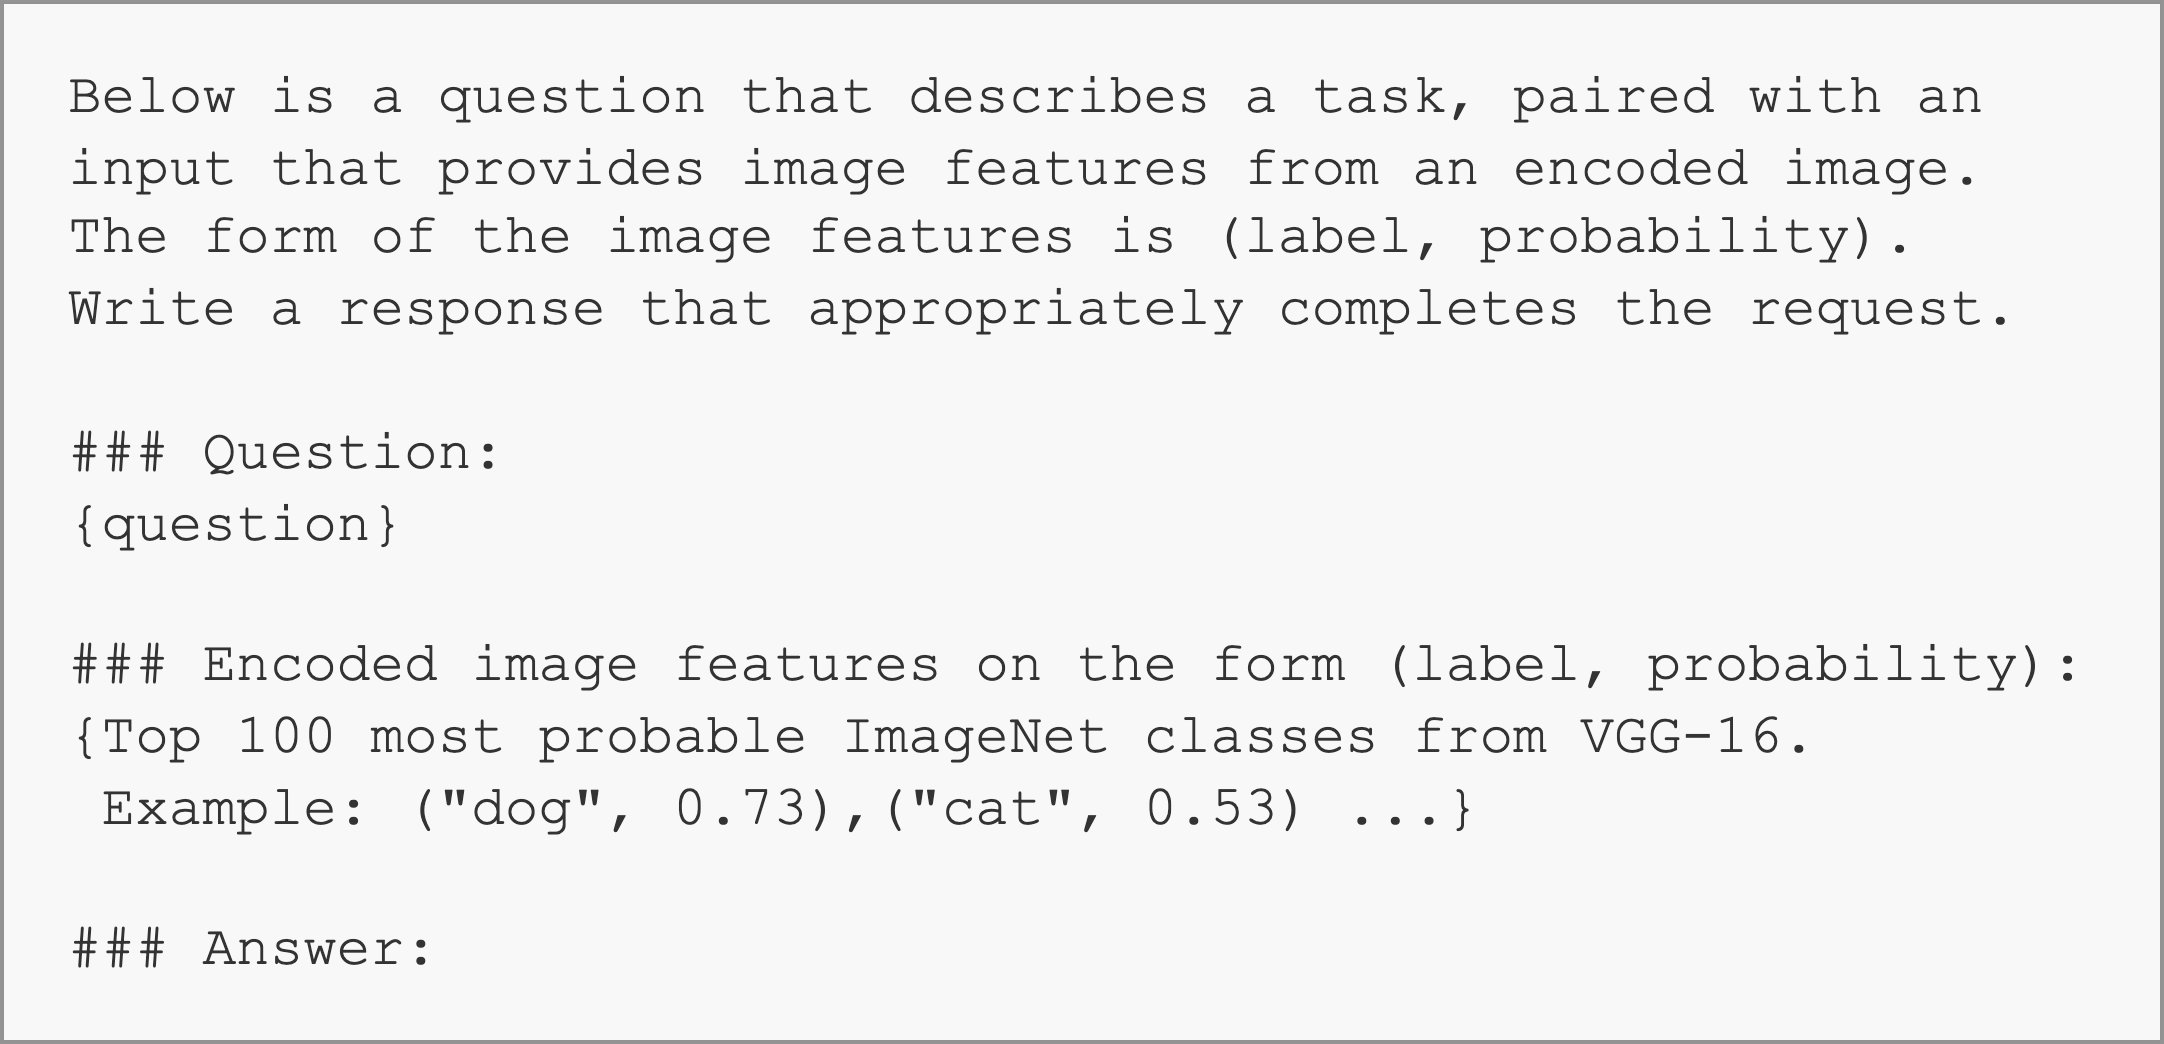
\includegraphics[width=\textwidth]{images/alpaca_modified_prompt_format.png}}
            \caption{Overview of the modified text prompt to the Alpaca-LoRA model, including extracted image features. The text in curly braces is not part of the prompt but represents the placeholder for the question and extracted image features.}
            \label{fig:alpaca_modified_prompt_format}
        \end{figure}



        

        \subsubsection{Text encoding}
        \label{sec3:text_encoding}
        % How to encode the text

        A text tokenization process is needed to break down the raw text data given in the prompt into smaller, standardized units called tokens, as described in Section \ref{sec2:text_tokenization}. 
        This process assures that text models, \glspl{llm}, in this case, can interpret linguistic input data. Tokenization is essential to transform unstructured text data into a format the model can process.
        
        \glspl{llm} have been trained on specific tokenization schemes that use unique tokenization rules and vocabularies. Therefore, they should use the same tokenizer when pre-training the model to get adequate performance. Suppose a different tokenizer is used to pre-process the text data. In that case, the tokenization output may not be compatible with the language model's vocabulary and encoding scheme, leading to poor model performance and incorrect predictions.
        
        Using the tokenizer from the language model was designed for ensures that the tokenization process is consistent with the training data and the model's internal encoding scheme. 
        This consistency ensures that the same tokenization scheme is used during both pertaining, fine-tuning, and inference. It is essential for the model consistency to learn the patterns and relationships within the text data effectively. 
    
        The tokenizer from the language model has been trained on a large corpus of text data and optimized to handle specific language patterns and nuances. This makes it more effective than tokenization schemes that may not have the same optimization and language-specific knowledge level. 
        Using the language model's tokenizer ensures that the text data is pre-processed in a way that is most compatible with the model, leading to better performance and more accurate predictions.

        The tokenizer used in this implementation is the one used by the original \gls{llama} model \cite{touvronLLaMAOpenEfficient2023} since the Alpaca model is a fork of this model. HuggingFace \cite{HuggingFaceAI} makes the specific implementation of the used LlamaTokenizer  and is based on SentencePiece \cite{LLaMATokenizer, Sentencepiece}. 
        This tokenizer and corresponding detokenizer allow for an unsupervised, end-to-end system without language-specific processing. 



        \subsection{Explaining the output}

        As \glspl{llm} are large and complex models, they can be challenging to explain. The model used in this experiment is small compared to other state-of-the-art \glspl{llm}, yet it consists of seven billion parameters, making it too large for many \gls{xai} methods. Explaining large transformer models is an area of research where many are working on developing new approaches. However, there is still no \textit{de facto} method to explain \glspl{llm}.

        % Attention and transition scores
        \subsubsection{Transition Scores and Attention}
        There are still various approaches to getting an explanation from transformers. The most popular method is to extract values from the attention weights of the transformer \cite{cheferGenericAttentionModelExplainability2021, cheferTransformerInterpretabilityAttention2021, barkanGradSAMExplainingTransformers2021, bohleHolisticallyExplainableVision2023}. Research has been done on finding subsets of the attention or even single neurons that are strongly associated with specific tasks, like the \textit{"sentiment neuron"} presented by Radford et al. \cite{radfordLearningGenerateReviews2017}. Here the researchers trained an \gls{lstm} on Amazon reviews to predict the next character of the text. When the model was trained, they made it into a sentiment classifier by adding a linear layer on top of the \gls{lstm}'s vector units. Available labeled sentiment data trained this linear layer. They noticed that one single neuron significantly impacted the predicted sentiment value. By dialing this single neuron, the sentiment of the text generated by the \gls{lstm} could be controlled. 
        
        However, the attention weights have proven unreliable as a factual explanation of what the model evaluates on a low-level \cite{serranoAttentionInterpretable2019, jainAttentionNotExplanation2019, abnarQuantifyingAttentionFlow2020}. 

        Although attention weights are not a reliable source of explanation, there still may be exciting insights to gain by analyzing these weights, as demonstrated by the \textit{"sentiment neuron"}.
        In this experiment, the transition scores of the \gls{llm} will be used to gain insight into how the implemented Alpaca-VQA model works. 
        These transition scores are calculated using its attention when the \gls{llm} predicts the next word in a sequence from the probability distribution. Although these scores do not give insight into the answer's validity, they indicate how sure the model is predicting the words.  


        % Proxy model
        \subsubsection{Proxy Model and LIME}
        Because of the size of \glspl{llm}, \gls{xai} methods such as \gls{lime} and \gls{shap} can be hard to implement to fit these large models or take a lot of time when finding perturbations on the input text and their corresponding output. Initial experiments with both \gls{lime} and \gls{shap} on the Alpaca-VQA model did not manage to make explanations because of the token size, making the run time unreasonably long.
        
        
        A proxy model was therefore developed to have a model that can shed light on how the input affects the output. 
        As \glspl{llm} are often complex and have millions or even billions of parameters, making their internal workings challenging to interpret. A simplified version that is easier to understand and explain can be created by training a proxy model on top of the large language model. This proxy model acts as a "translator" between the complex language model and human interpreters, providing a more interpretable representation of the underlying model's decision-making process.
        The proxy model can help address the issue of transparency and trust in \gls{ai} systems. Like many deep neural networks, \glspl{llm} are often treated as black boxes, where the input-output relationship is not easily interpretable. By training a proxy model, insights can be gained into how the language model makes decisions, and this insight can be achieved using techniques such as \gls{lime}. 
        These explanations can help users understand why the model made a particular decision and provide a level of transparency and trust in the system.
        Therefore, training a proxy model on a large language model enables us to bridge the gap between the complexity of the underlying model and the need for interpretability and explainability.

        The proxy model used to mimic and interpret the Alpaca-VQA model is a \gls{sdg} classifier. 
        The data used to train the classifier includes 14,000 question-answer pairs, with the appropriate answers provided by Alpaca-VQA. The model is trained on the response predicted by the \gls{llm} instead of the ground truth to predict the same as the Alpaca-VQA. With 20,000 question-answer pairs created by the \gls{llm}, divided into 14,000 in the training set and 6,000 in the test set, the \gls{sdg} classifier achieves an accuracy of 86\% in the test set.
        
        This proxy model is then fitted with the \gls{lime} method to make it explainable. Since \gls{lime} fits a linear model to the model it explains, there are three stacked models in total in the explanation pipeline, as seen in Figure \ref{fig:LIMEpyramide}. 
        Even though stacked models obscure the actual decisions of the underlying model, some valuable insights can still be gained. 
        Despite fitting a proxy model itself, the \gls{lime} method has proven effective in providing insight into the inner workings of numerous models. Therefore, this experiment will test whether an additional proxy model would provide valuable explanations or insights into the Alpaca-VQA model. 
         

        \begin{figure}[htb]
            \centering
            \centerline{
            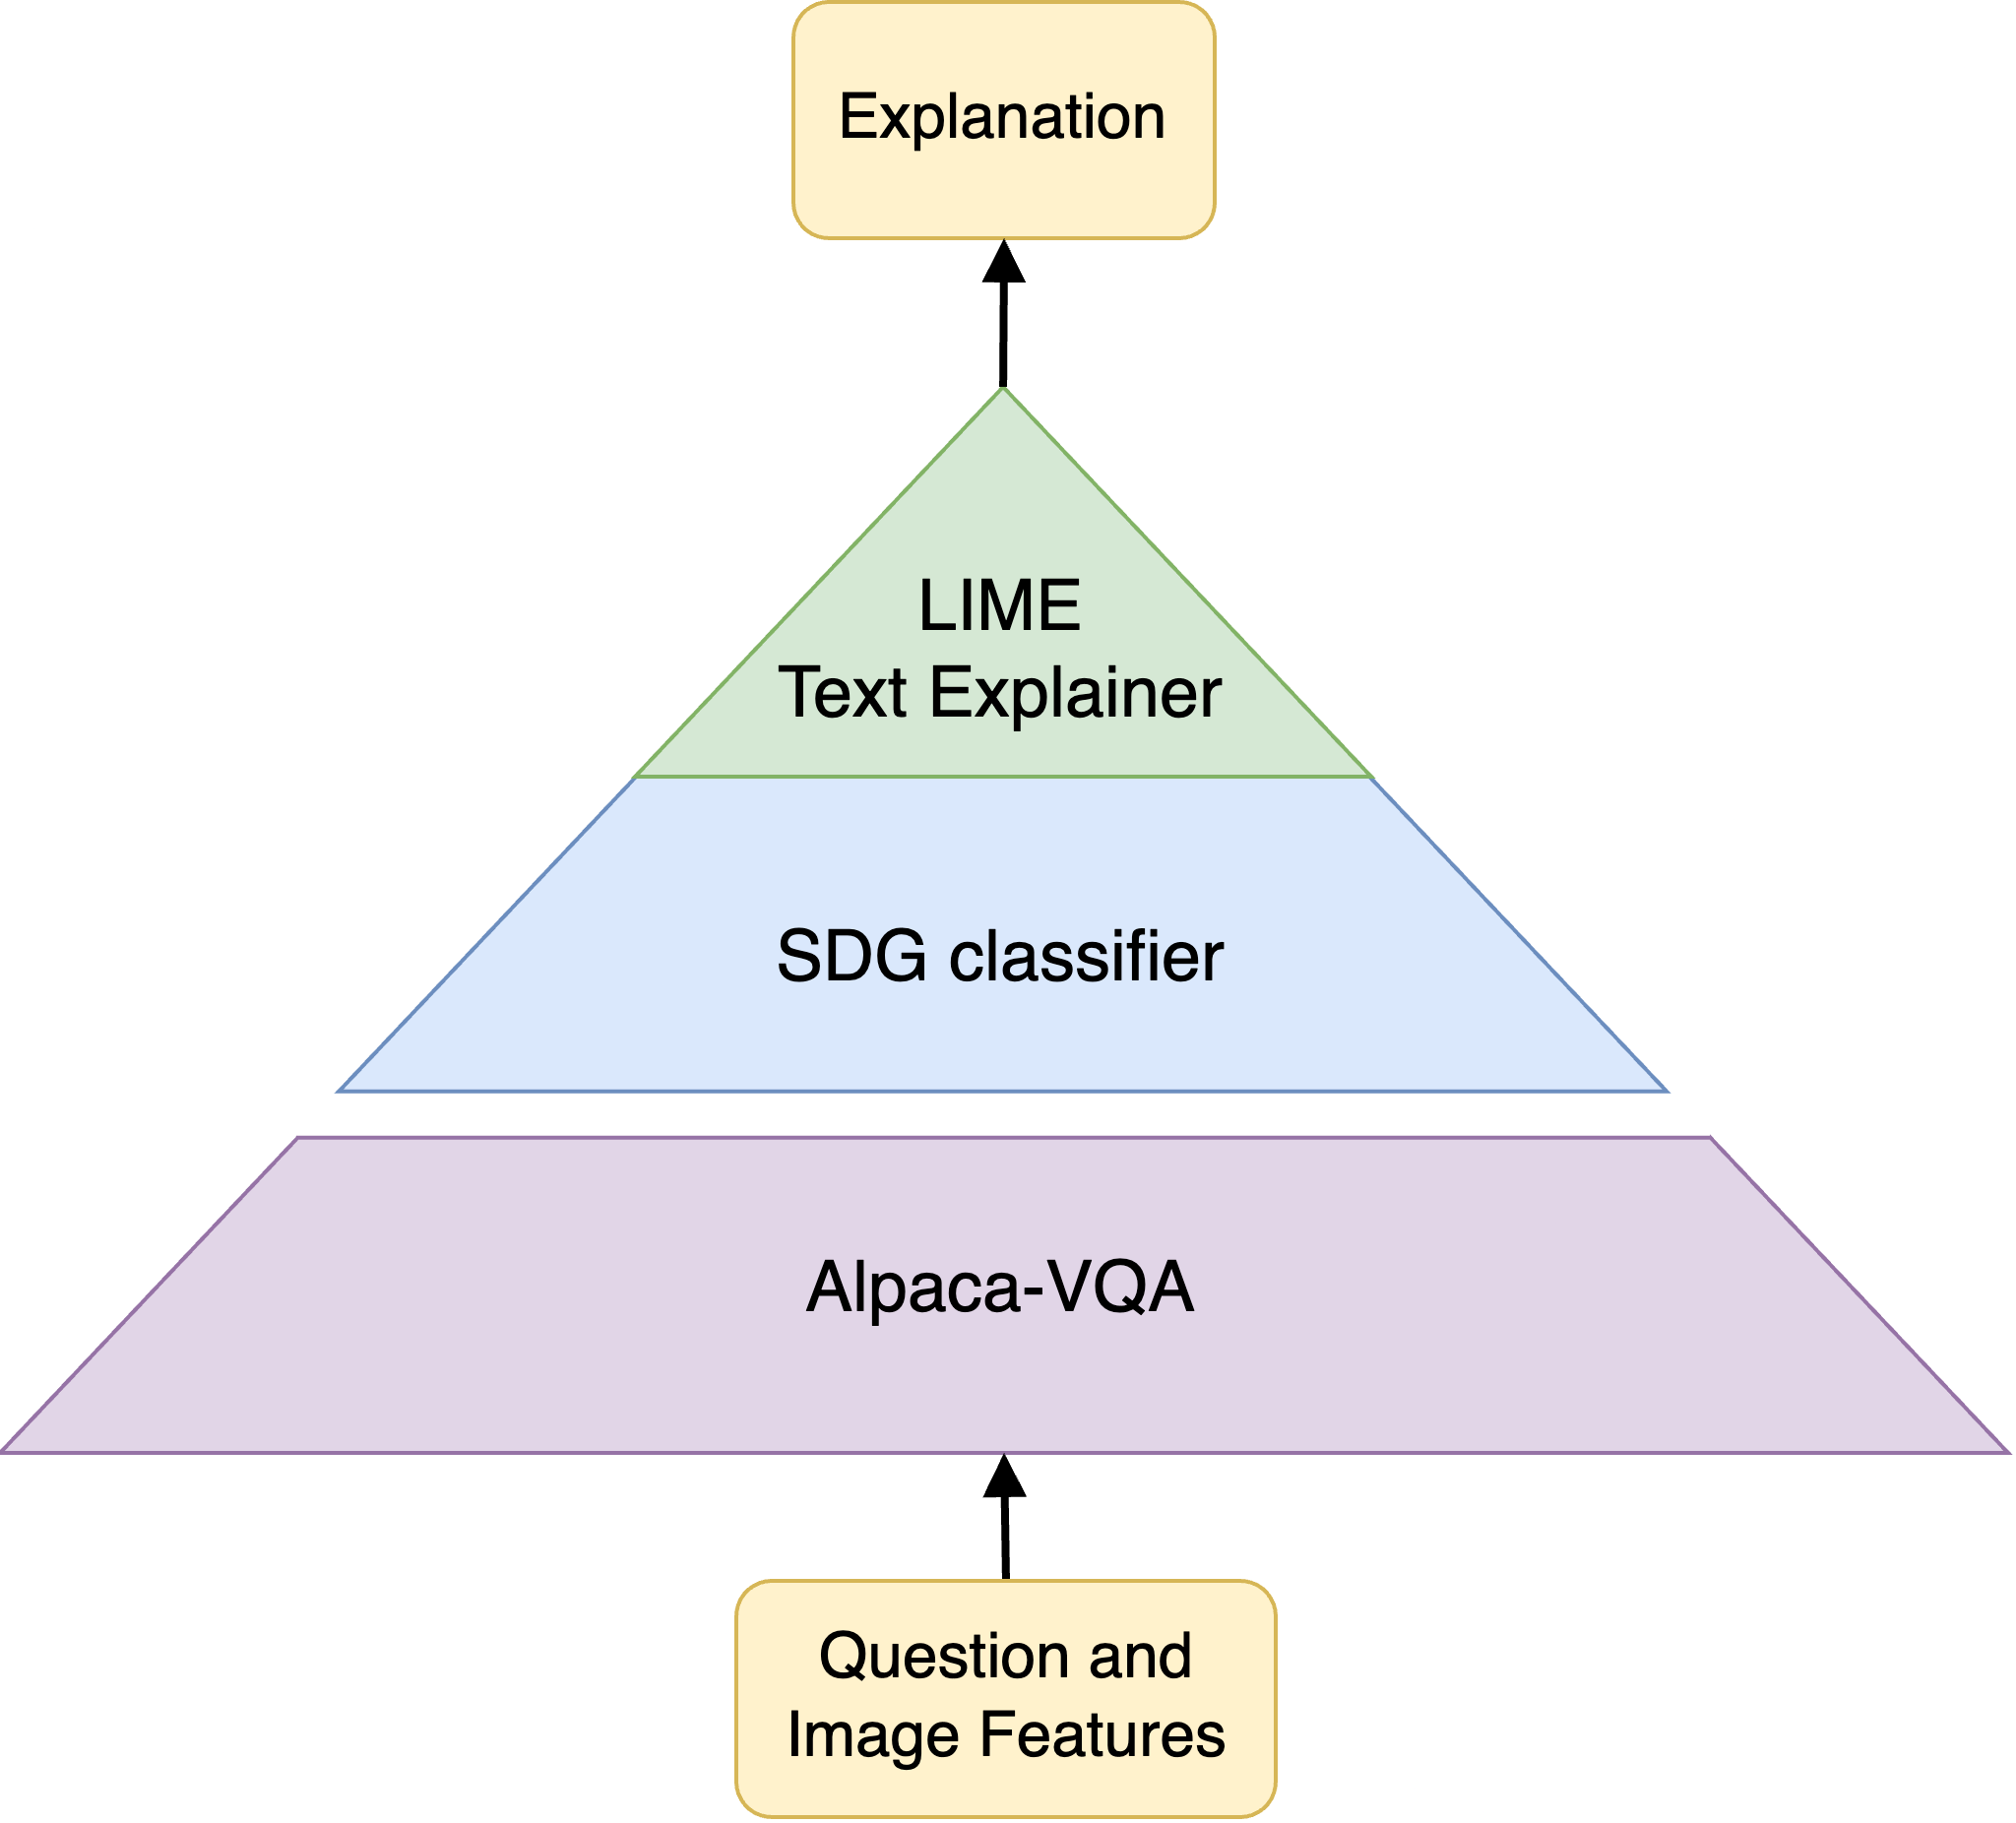
\includegraphics[width=11cm]
            {images/LIMEpyramide.png}}
            \caption{This figure represents the explanation pipeline of the Alpaca-VQA model using a proxy model that is explained by \gls{lime}. The question and image features are fed into Alpaca-VQA, which predicts an answer. This answer is used to train a \gls{sdg} classifier that gets explained by \gls{lime}.}
            \label{fig:LIMEpyramide}
        \end{figure}


        
        
        

    % Dataset
    \subsection{Dataset}
        
        The images used in this experiment are from the \textit{HyperKvasir} developed by Borgli et al. \cite{borgliHyperKvasirComprehensiveMulticlass2020}, and the VQA extension using these images from the \textit{ImageCLEFmed-MEDVQA-GI-2023} dataset by Hicks et al. \cite{hicksImageCLEFmedMEDVQAGI20232023, hicksImageCLEFmedMEDVQAGIImageCLEF}. 
        
        \subsubsection{HyperKvasir}
        The available dataset on the gastrointestinal tract is one of the most extensive datasets, which comprises images and videos. The data was collected during examinations at Bærum Hospital in Norway, including anatomical landmarks and normal pathological findings.
        A subset of the images and videos were annotated by at least one experienced gastroenterologist, from Bærum Hospital, the Cancer Registry of Norway, or Karolinska University Hospital in Sweden, together with one or more experienced persons working in the medical field.  
        
        The dataset can benefit medical and technical communities exploring semi-supervised and unsupervised methods. It can also help artificial intelligence-based computer-assisted diagnosis systems to provide better patient treatment.
        The full HyperKvasir dataset is available to the public and is open access\footnote{https://doi.org/10.17605/OSF.IO/MH9SJ, https://datasets.simula.no/hyper-kvasir}.


      
        \subsubsection{ImageCLEFmed-MEDVQA-GI-2023}

        This dataset extends HyperKvasir by adding multiple modalities to a subset of the images, specifically \gls{vqa}, Visual Question Generation (VQG), and Visual Location Question Answering (VLQA).
        The dataset is developed for the CLEF 2023 Medical Visual Question Answering (MedVQA) Challenge and is available to the public \footnote{https://github.com/simula/ImageCLEFmed-MEDVQA-GI-2023}.
        
        The  question-and-answer ground truth is developed with medical partners, and the data include images spanning the entire gastrointestinal tract. Questions and answers include abnormalities, surgical instruments, and normal findings. 
        
        Since the experiments in this thesis are based on \gls{vqa}, the questions regarding \gls{vqa} in this dataset were used. To test if the \gls{llm} could learn some location capabilities, even though the \gls{cnn} does not output bounding boxes, the questions regarding the location were also included. 
        

        \subsubsection{Dataset Preparation}
        
        The original dataset is structured as a nested JSON file, and the structure can be seen in Figure \ref{fig:colon_vqa_original_json}.
        It is structured to have the image ID as the key and related questions and answers as value. The input text prompt to the model must have the image data, question, and answer bundled together in each prompt, as seen in Figure \ref{fig:alpaca_modified_prompt_format}, the data structure was unrolled. 


        \begin{figure}[htb]
            \centering
            \centerline{
            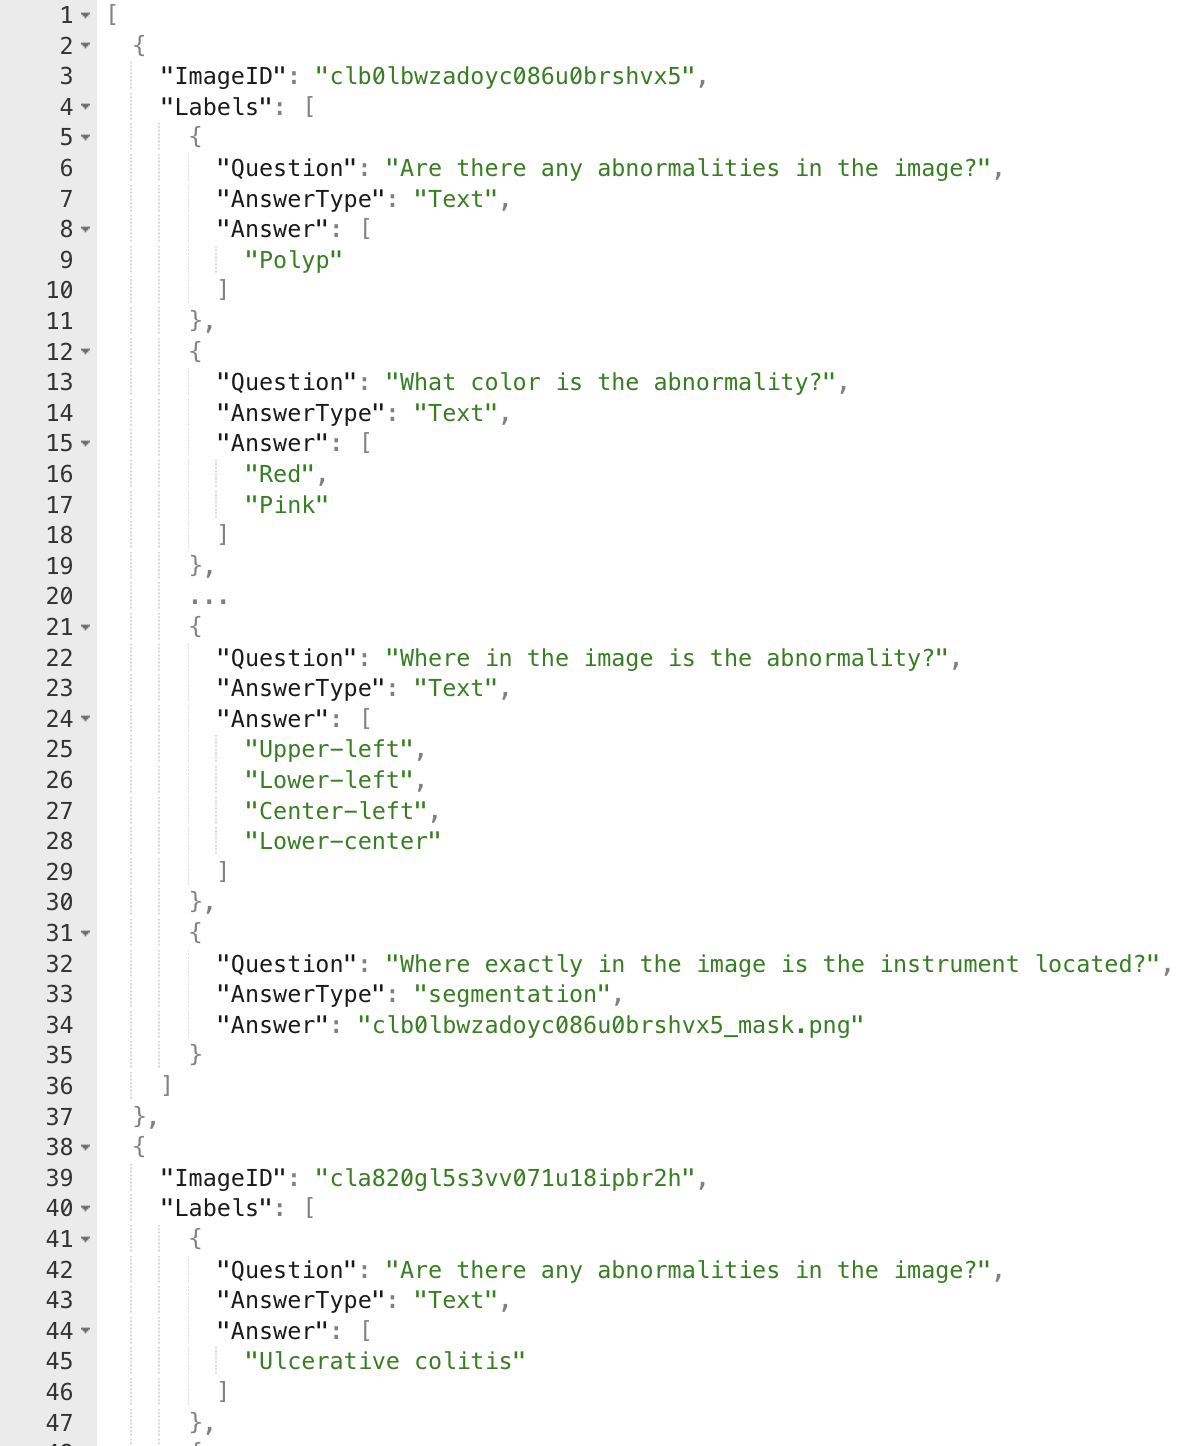
\includegraphics[width=1.2\textwidth]{images/colon_vqa_original_json.png}}
            \caption{The original JSON from the ImageCLEFmed-MEDVQA-GI-2023 dataset. It comprises 6683 question-answer pairs related to images in a nested structure, with the image ID as the key and the question-answer pairs as values.}
            \label{fig:colon_vqa_original_json}
        \end{figure}


        First, the nested structure was flattened so each row received the appropriate image ID, making the prompts easier to parse. The resulting structure can be seen in Figure \ref{fig:colon_vqa_pandas}. However, some questions, particularly regarding localization and color, have multiple correct answers. Instead of teaching the model to score multiple correct answers, the questions were flattened. Evaluating multiple correct answers to a question can be challenging because the model needs to know which answer is correct and which is incorrect. To circumvent this challenge, the answers in the dataset are flattened so that each row contains only one correct answer.

        \begin{figure}[htb]
            \centering
            \centerline{
            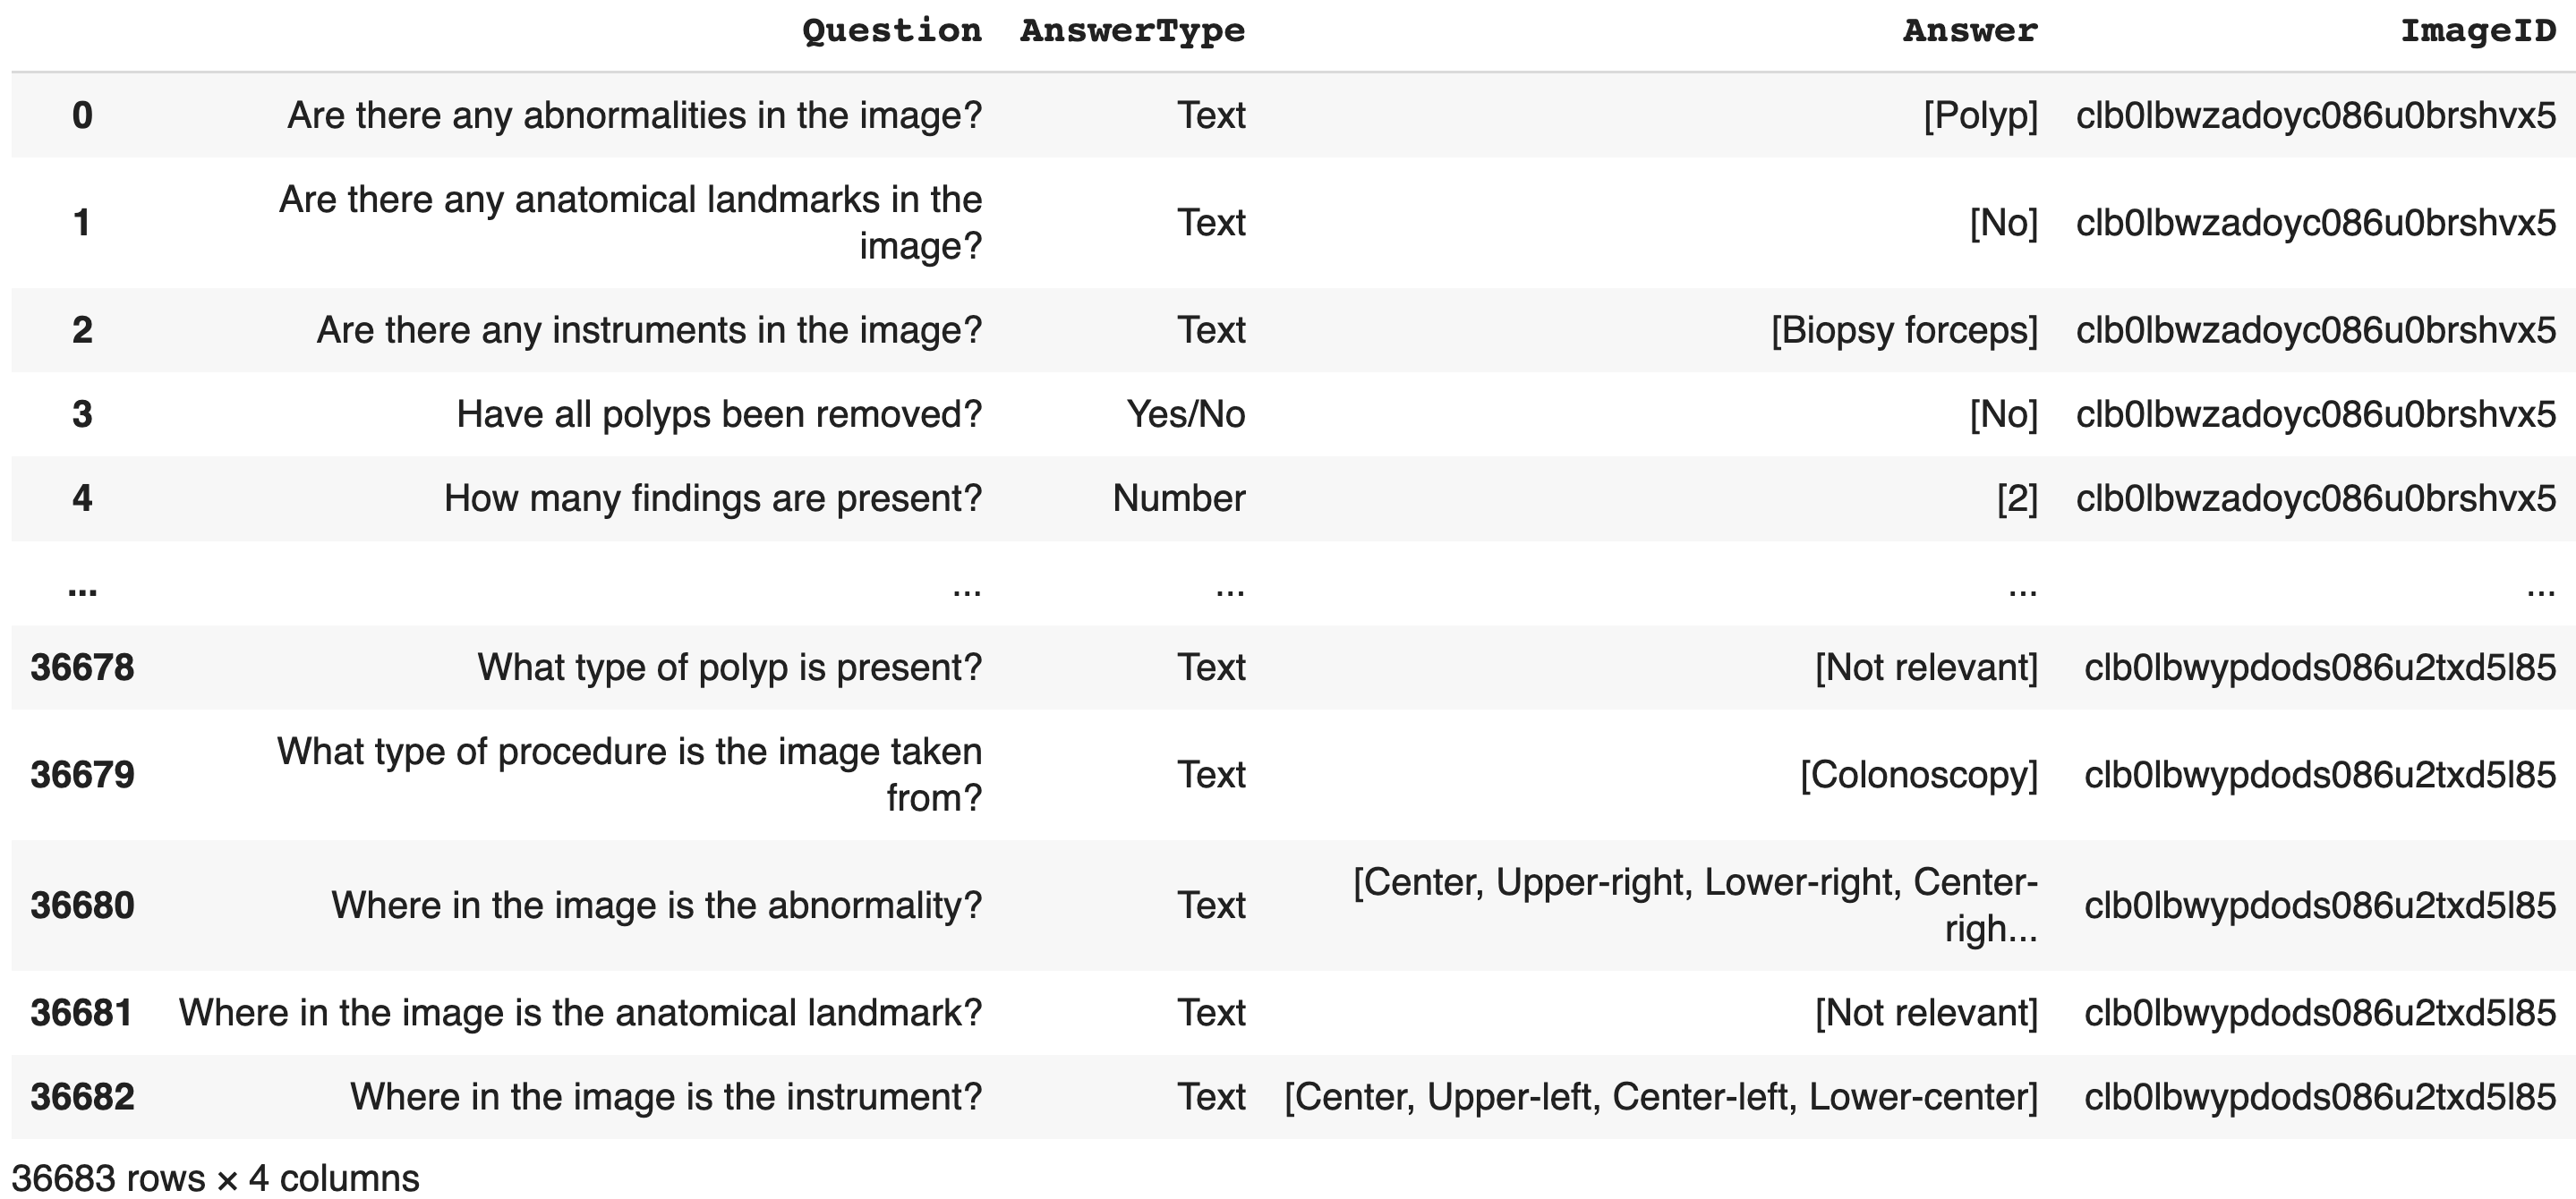
\includegraphics[width=1.2\textwidth]{images/colon_vqa_pandas.png}}
            \caption{The ImageCLEFmed-MEDVQA-GI-2023 has the image IDs flattened. In this structure, each row has a question-answer pair and a corresponding image ID. Responses are still grouped in a list, making it difficult to evaluate individual responses.}
            \label{fig:colon_vqa_pandas}
        \end{figure}

        Having all information self-contained would make inputting one row into the prompt easier, as all necessary information is contained in the row. 
        When the \gls{llm} predicts an answer, it can be quickly compared to the ground truth, making calculating accuracy more straightforward.
        This flatting of ground truth answers made the original 36'683 question-answer pairs into 52'051 pairs.
        The final structure of the data used in this experiment can be seen in Figure \ref{fig:colon_vqa_pandas_exploded}.

        \begin{figure}[htb]
            \centering
            \centerline{
            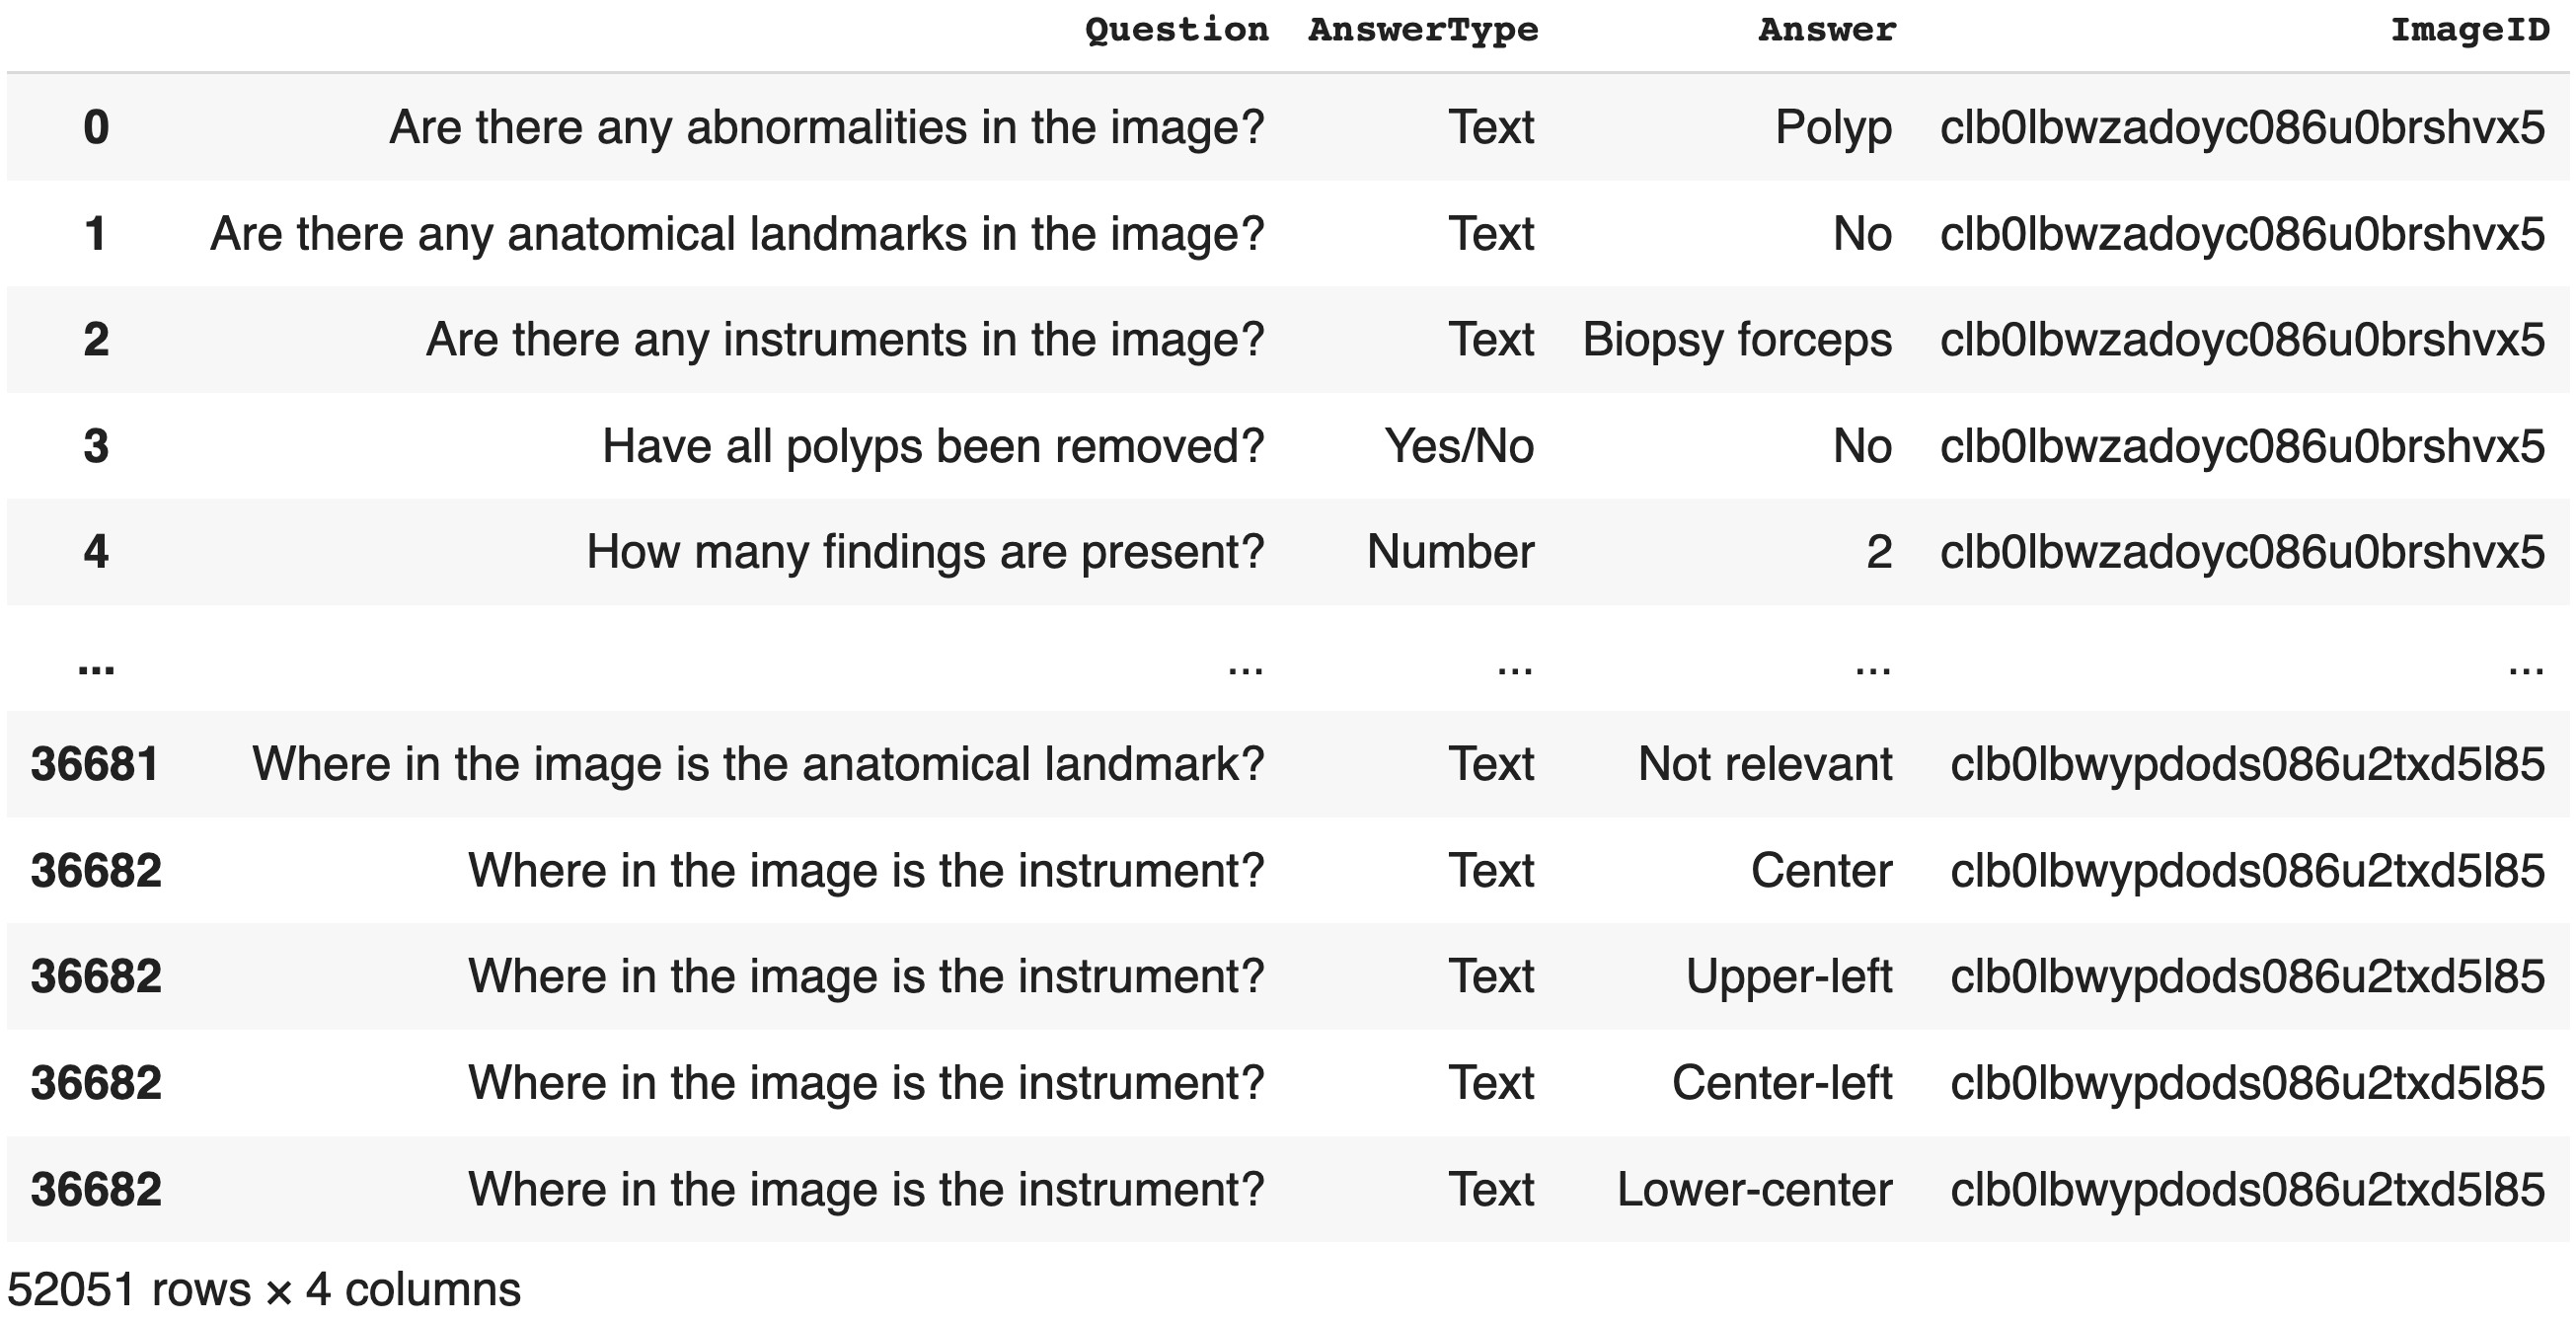
\includegraphics[width=1.2\textwidth]{images/colon_vqa_pandas_exploded.png}}
            \caption{The ImageCLEFmed-MEDVQA-GI-2023 with image IDs and answers flattened. This structure has one question-answer pair on each row, allowing for easier calculation of predictions. This is the structure used when training the model in this experiment.}
            \label{fig:colon_vqa_pandas_exploded}
        \end{figure}

        
        
    \subsection{Context Window, Cuttoff, and Evaluation Metrics}
         This section will discuss essential features when training language models: context window, cutoff length, and evaluation metrics. 

        % How to train the model
        \subsubsection{Context window and cutoff length}
        \label{sec:3_cutoff}
        The context window of a language model refers to the number of words or tokens considered in predicting the next word or token. The context window is typically linked to both the input prompt and the output since the model refers to the input when generating the output. When training \glspl{llm}, the model receives a sequence of input tokens and produces a series of output tokens. 
        Similarly, when fine-tuning a pre-trained language model on a specific task, the context window is also linked to both the input and the output. 
        The input would consist of the prompt defined by the context window, and the output would be the predicted tokens that the \gls{llm} predicts based on the tokens in the context window. 
        By adjusting the context window size, researchers can control the amount of context the model uses to generate its predictions, which can impact its accuracy and efficiency.

        % how context window and cutoff length are related 
        Cutoff length is a term often used when fine-tuning a pre-trained language model. The cutoff length specifies the maximum length of the prompt used when generating an answer.

        Therefore, the context window and the cutoff length are closely related features that should be considered in conjunction. In practice, the context window can be regarded as a way to capture longer-term dependencies between words in a sequence. At the same time, the prompt cutoff length imposes a constraint on the size of input the model should process for a given task.
        

        % Specific cutoff length
        The updated input prompt shown in Figure \ref{fig:alpaca_modified_prompt_format} was used to training the model to interpret images. The prompt cutoff length was updated from the original 256 to 1485 tokens. The original LLaMA model was trained on 2048 tokens \cite{SequenceContextLength}, and the original Alpaca model is fine-tuned with 512 tokens as the cutoff length. The authors of the model used in this experiment, Alpaca-LoRA, analyzed the training data and found that 96\% of the prompts could be answered using a cutoff length of 256 tokens. 
        When deciding on the new token length, including the top 100 classes from \gls{vgg}-16, the LlamaTokenizer must encode the whole input text, including image features.  
        
        When the class prediction score was represented using Numpy's floating number with 32 bits of precision, the average token length of just the image features where 162'654. As this would increase the original token size by more than 63,000\%, it was considered too significant to be reasonable for the model. Because the used language model uses the LoRA technique to lower memory consumption, such a considerable cutoff length should still technically be feasible. However, the increased training and inference time was considered too inefficient for this experiment.  
        The prediction score was converted to floats with 16 bits of precision to decrease the image token length. In practice, this would not make a difference in accuracy when fed into the language model, as the predicted class is just a placeholder for the underlying feature maps extracted. 
        The advantage of converting the prediction score is that the average token length of the extracted 100 classes was reduced to 144'654 tokens. The reduced token size is an 11\% reduction of tokens from the 32-bit precision representation and would still benefit from a further reduction. 
        To give an additional decrease in the length of the prediction scores, they were rounded to three decimals. This will still provide the language model insight into the extracted class labels and the relationship between the classes while also significantly reducing the prediction score token length. 
        The final rounded scores have an average length of 1229 tokens, resulting in a reduction of 99\% from the original 32-bit precision score. 
        Combined with a prompt text length of 256, the total cutoff length is therefore calculated to be 1485 tokens. 
        Thus, this cutoff length is designed to cover 96\% of the original prompts while incorporating the 100 most probable classes and their predictions. 

         


        \subsubsection{Evaluation metrics}
        % Evaluation metrics used
        The evaluation metrics used in the Alpaca-VQA model experiments are precision, recall, accuracy, and $F_1$ score. These metrics are defined in detail in Section \ref{sec2:performance_metrics}.
        
        The precision is used to evaluate the proportion of the correct predicted classes, and the recall is used to see how well the model predicts correct classes.
        $F_1$ score is used to find the harmonic mean of the model's precision and recall and is a combined score of these two metrics. This score is used to more easily compare the score of each class in the test dataset. 
        Accuracy is used to see how well the model predicts the correct classes. 
        
        Lastly, perplexity is used as a metric to analyze how well the model predicts an answer, given its probability distribution. 
        The features from this perplexity calculation are also used to calculate a prediction score for each token in the answer. This gives insight into how sure the model is about its prediction.
       
        

        % Summary
        

% SUMMARY:
\section{Summary}

In summary, this chapter has discussed the methods used when developing the two approaches to explain \gls{vqa} tasks. These two models investigate explanations originating from different domains.


The first proposed method, FLEX-VQA, combines the \gls{flex} framework with \gls{vqa} to explain the network's visual reasoning to explain why an answer to an image-question pair is using natural language. 
The Alpaca model was chosen for this experiment as it was already pre-trained and required less computing power than other \glspl{llm}. The \gls{lora} technique was used to fine-tune the Alpaca model further, which adds pairs of rank-decomposition weight matrices on the current weights and only trains these newly added weights. This approach accelerates the training while reducing memory consumption, making training domain-specific models more feasible and faster.
The image features of the \gls{cnn} are translated into text, and the explanation happens in the text domain of the \gls{llm} using \gls{lime} and transition scores.


The next chapter will present the results achieved with the Alpaca-VQA, as the FLEX-VQA method was unfeasible to run because of outdated frameworks. 
The results gained from the Alpaca-VQA will be explained, discussed, and compared.